%%%%%%%%%%%%%%%%%%%%%%%%%%%%%%%%%%%%%%%%%%%%%%%%%%%%%%%%%%%%%%%%%%%%%%%%%%%%%%%
%%                                                                           %%
%%   Dr Varun Ojha                                                           %%
%%   Lecturer, Department of Computer Science                                %% 
%%   University of Reading, UK                                               %%
%%                                                                           %%
%%%%%%%%%%%%%%%%%%%%%%%%%%%%%%%%%%%%%%%%%%%%%%%%%%%%%%%%%%%%%%%%%%%%%%%%%%%%%%%
%%%%     SETTING STARTS - DO NOT CHANGE Unless your TeX setting require so   %%
%%%%%%%%%%%%%%%%%%%%%%%%%%%%%%%%%%%%%%%%%%%%%%%%%%%%%%%%%%%%%%%%%%%%%%%%%%%%%%%
%%----------------------------------------------------------------------------------
% DO NOT Change this. It is the required setting A4 page, 11pt, onside print, book style
%%----------------------------------------------------------------------------------
\documentclass[a4paper,11pt,oneside]{book}

%%-------------------------------------
%% Page margin settings - % half inch margin all sides (recommended)
%%-------------------------------------
\usepackage[margin=1.2in]{geometry} 

%%-------------------------------------
%% Font settings - % CM San or Ariel (recommended)
%%-------------------------------------
% Switch the following two line off: to revert back to default LaTex font (NOT recommended)
\usepackage{amsfonts}
\renewcommand*\familydefault{\sfdefault}

%%-------------------------------------
%% Math/Definition/Theorem/Algorithm packages settings 
%%-------------------------------------
\usepackage[cmex10]{amsmath}
\usepackage{amssymb}
\usepackage{amsthm}
\newtheorem{mydef}{Definition}
\newtheorem{mytherm}{Theorem}

% \usepackage{subcaption}

\usepackage{makecell}

%%-------------------------------------
%% Algorithms/Code Listing environment settings  - 
%% Please do not change these settings
%%-------------------------------------
\usepackage{algorithm}
\usepackage{algpseudocode}
\renewcommand{\algorithmicrequire}{\textbf{Input:}}
\renewcommand{\algorithmicensure}{\textbf{Output:}}
\usepackage[utf8]{inputenc}
\usepackage{listings}
\usepackage{xcolor}
\definecolor{codegreen}{rgb}{0,0.6,0.1}
\definecolor{codegray}{rgb}{0.5,0.5,0.5}
\definecolor{codeblue}{rgb}{0.10,0.00,1.00}
\definecolor{codepurple}{rgb}{0.58,0,0.82}
\definecolor{backcolour}{rgb}{1.0,1.0,1.0}

\lstdefinestyle{mystyle}{
    backgroundcolor=\color{backcolour},   
    commentstyle=\color{codegreen},
    keywordstyle=\color{codeblue},
    numberstyle=\tiny\color{codegray},
    stringstyle=\color{codepurple},
    basicstyle=\ttfamily\footnotesize,
    breakatwhitespace=false,         
    breaklines=true,                 
    captionpos=b,                        
    keepspaces=true,                 
    numbers=left,                    
    numbersep=5pt,                  
    showspaces=false,                
    showstringspaces=false,
    showtabs=false,                  
    tabsize=2,
    frame=none
}
\lstset{style=mystyle}

%%-------------------------------------
%% Graphics/Figures environment settings
%%-------------------------------------
\usepackage{graphicx}
\usepackage{subfigure}
\usepackage{caption}
\usepackage{lipsum}

\usepackage{pgffor}

\usepackage[section]{placeins}
\usepackage{multirow}

%%-------------------------------------
%% Table environment settings
%%-------------------------------------
\usepackage{multirow}
\usepackage{rotating}
\usepackage{makecell}
\usepackage{booktabs}
%\usepackage{longtable,booktabs}

%%-------------------------------------
%% List of Abbreviations settings
%%-------------------------------------
\usepackage{enumitem}
\newlist{abbrv}{itemize}{1}
\setlist[abbrv,1]{label=,labelwidth=1in,align=parleft,itemsep=0.1\baselineskip,leftmargin=!}

%%-------------------------------------
%% Bibliography/References settings   - Harvard Style was used in this report
%%-------------------------------------
\usepackage[hidelinks]{hyperref}
\hypersetup{ 
    colorlinks=true, 
    linkcolor=blue, 
    filecolor=blue, 
    citecolor = black,       
    urlcolor=cyan, 
 } 
\usepackage[comma,authoryear]{natbib}
\renewcommand{\bibname}{References} % DO NOT remove or switch of 

%%-------------------------------------
%% Appendix settings     
%%-------------------------------------
\usepackage[toc]{appendix}
%%%%%%%%%%%%%%%%%%%%%%%%%%%%%%%%%%%%%%%%%%%%%%%%%%%%%%%%%%%%%%%%%%%%%%%%%%%%%%%%%%%%%%%
%%%%                     SETTING ENDS                                            %%%%%%
%%%%%%%%%%%%%%%%%%%%%%%%%%%%%%%%%%%%%%%%%%%%%%%%%%%%%%%%%%%%%%%%%%%%%%%%%%%%%%%%%%%%%%%
\begin{document}

    \captionsetup[figure]{margin=1.5cm,font=small,name={Figure},labelsep=colon}
    \captionsetup[table]{margin=1.5cm,font=small,name={Table},labelsep=colon}
    % \setlipsumdefault{1}
    
    \frontmatter
    
    \begin{titlepage}      
        \begin{center}
            
\includegraphics[width=3cm]{figures/figures_misc/uorlogo.png}\\[0.5cm]
            {\LARGE University of Reading\\[0.5cm]
            Department of Computer Science}\\[2cm]
			%{\color{blue} \rule{\textwidth}{1pt}}
			
			% -------------------------------
			% You need to edit some details here
			% -------------------------------  
            \linespread{1.2}\huge {
                %%%%%%%%%%%%%%%%%%%%%%%%%%%%
                %TODO: 1 TITLE of Your PROJECT 
                %%%%%%%%%%%%%%%%%%%%%%%%%%%%
                % chnage the following line                
                Generating Tree Genus Classification and Change Maps to Assist Mitigate Climate Change
            }
            \linespread{1}~\\[2cm]
			%{\color{blue} \rule{\textwidth}{1pt}}
            {\Large 
                %%%%%%%%%%%%%%%%%%%%%%%%%%%%
                %TODO: 2 YOUR NAME
                %%%%%%%%%%%%%%%%%%%%%%%%%%%%             
                % chnage the following line
                Pedro Junio
                % change end             
            }\\[1cm] 
            

            {\large 
                %%%%%%%%%%%%%%%%%%%%%%%%%%%%
                %TODO: 3 YOUR NAME Supervisor's name(s)
                %%%%%%%%%%%%%%%%%%%%%%%%%%%%             
                % change the following line                
                \emph{Supervisor:} Muhammad Shahzad}\\[1cm] % if applicable
            
    		% PLEASE DO NOT CHANGE THIS TEXT %
            \large A report submitted in partial fulfillment of the requirements of\\the University of Reading for the degree of\\ Master of Science in \textit{Data Science and Advanced Computing}\\[0.3cm] 
            \vfill
            
            \today 
        \end{center}
    \end{titlepage}
    % -------------------------------------------------------------------
    % Declaration
    % -------------------------------------------------------------------
    \newpage
    \thispagestyle{empty}
    \chapter*{\Large Declaration}
    % PLEASE CHANGE THIS TEXT EXCEPT YOUR NAME%
    % -------------------------------
    %TODO: PLEASE ONLY UPDATE HERE -- PLEASE WRITE YOUR NAME %    
    % ------------------------------- 
    I,
    %%%%%%%%%%%%%%%%%%%%%%%
    Pedro Junio, % Mandatory part
    %%%%%%%%%%%%%%%%%%%%%%%
    of the Department of Computer Science, University of Reading, confirm that this is my own work and figures, tables, equations, code snippets, artworks, and illustrations in this report are original and have not been taken from any other person's work, except where the works of others have been explicitly acknowledged, quoted, and referenced. I understand that if failing to do so will be considered a case of plagiarism. Plagiarism is a form of academic misconduct and will be penalised accordingly. \\
    
    %% Please delete as appropriate. 
    \noindent
    %%%%%%%%%%%%%%%%%%%%%%%%%%%%%%%%%%%%%%%%%%%%%%% 
    %TODO 1 Consent for example copy -  we will use 
    I give consent to a copy of my report being shared with future students as an exemplar. \\
    
    \noindent
    %%%%%%%%%%%%%%%%%%%%%%%%%%%%%%%%%%%%%%%%%%%%%%% 
    %TODO 2 Consent to let the report to use use by library for public use
    I give consent for my work to be made available more widely to members of UoR and public with interest in teaching, learning and research. 
    %%%%%%%%%%%%%%%%%%%%%%%%%%%%%%%%%%%%%%%%%%%%%%%
    ~\\[1cm]
    \begin{flushright}
	%------------------------------ 
	% change the following line
    %TODO: PLEASE UPDATE  Your Name  -------------------------------%
	Pedro Junio % Please change it to your name
    
    \today
    \end{flushright}
    %Two resources useful for abstract writing.
% Guidance of how to write an abstract/summary provided by Nature: https://cbs.umn.edu/sites/cbs.umn.edu/files/public/downloads/Annotated_Nature_abstract.pdf %https://writingcenter.gmu.edu/guides/writing-an-abstract
\chapter*{\center \Large  Abstract}
%%%%%%%%%%%%%%%%%%%%%%%%%%%%%%%%%%%%%%
% Replace all text with your text
%%%%%%%%%%%%%%%%%%%%%%%%%%%%%%%%%%%
TODO update at the end

Variety of tree species are crucial in reducing the vulnerabilities and offering stable ecosystem functioning. The precise quantification and assessment of existing tree species on global-scale is therefore essential in filling the science-policy gaps by providing key insights essential in promoting the success of natural climate solutions and devising effective climate mitigation policies. To this end, this study aims to develop novel deep learning based algorithms by using the multi-temporal multi-spectral imagery to generate large-scale forest/tree species classification maps.

%%%%%%%%%%%%%%%%%%%%%%%%%%%%%%%%%%%%%%%%%%%%%%%%%%%%%%%%%%%%%%%%%%%%%%%%%s
~\\[1cm]
\noindent % Provide your key words
\textbf{Keywords:} Convolutional Neural Network, Sentinel-2, Copernicus, SoilGrid, EU-Forest, Forests, Tree Genera, Climate

\vfill
\noindent
\textbf{Report's total word count:} over 9000
    
    \tableofcontents
    \listoffigures
    \listoftables
    % \input{chapters/glossaries} %  Enter your list of Abbreviation and Symbols in this file
    
    %%%%%%%%%%%%%%%%%%%%%%%%%%%%%%%%%%%%%%%%%%%%%%%%%%%%%%%%%%%%%%%%%%%%%%%%
    %%                                                                    %%  
    %%  Main chapters and sections of your project                        %%  
    %%  Everything from here on needs updates in your own words and works %%
    %%                                                                    %%
    %%%%%%%%%%%%%%%%%%%%%%%%%%%%%%%%%%%%%%%%%%%%%%%%%%%%%%%%%%%%%%%%%%%%%%%%
    \mainmatter
   
    \chapter{Data Exploration}
\label{chapter:data}
\section{EU-Forest Labels}

\begin{figure}[!thb]
    \centering
    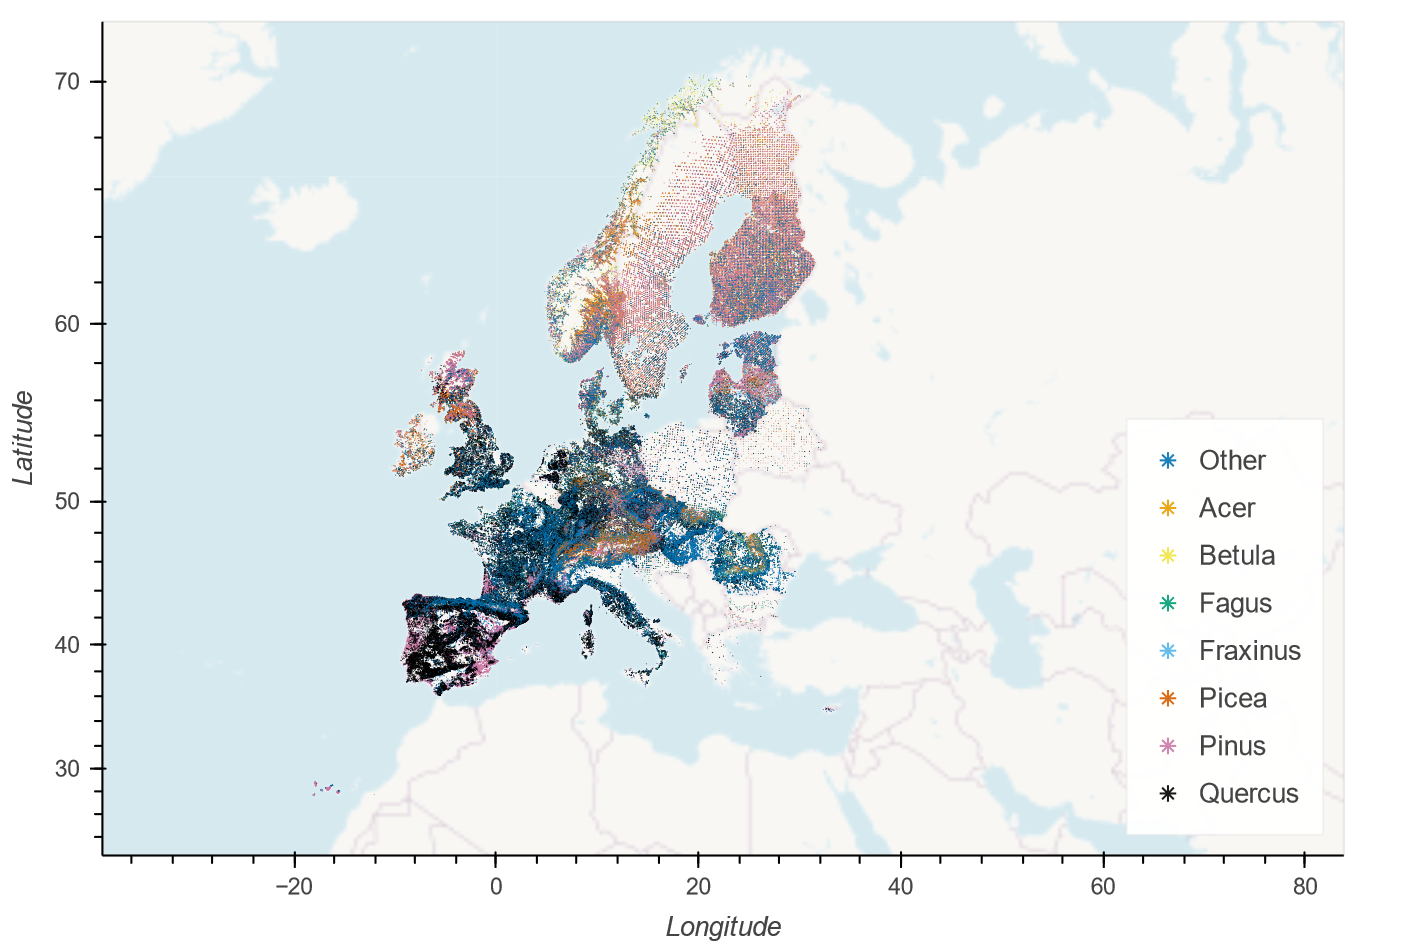
\includegraphics[width=0.9\linewidth]{figures/figures_labels/genus_cutoff_map.png}
    \caption{Map of the most common tree genera in EU-Forest.}
    \label{fig:genus_cutoff_map}
\end{figure}

EU-Forest is a dataset containing tree species and genera for nearly $250,000$ locations across Europe \cite{eu_forest_data}. Each plot is 1\,km\,×\,1\,km and may contain multiple tree species and genera. Fig.\,\ref{fig:genus_cutoff_map} shows the distribution of tree genera in the EU-Forest dataset across 21 European countries. In this figure, the label 'Other' is an umbrella class for 70 tree genera with less than 20,000 occurrences each.

Using the EU-Forest dataset to train a CNN classifier of tree genera with Sentinel-2 data offers several significant advantages. Firstly, the dataset's high spatial resolution enables fine-grained 
analysis of tree species distribution, which enhances the accuracy of the classifier. Its comprehensive coverage across Europe, including diverse forest types and geographical areas, allows the model to learn from a wide variety of environments and tree genera. The rich occurrence data provides detailed information on tree species, aiding in precise identification and classification.

\begin{figure}[!thb]
    \centering

    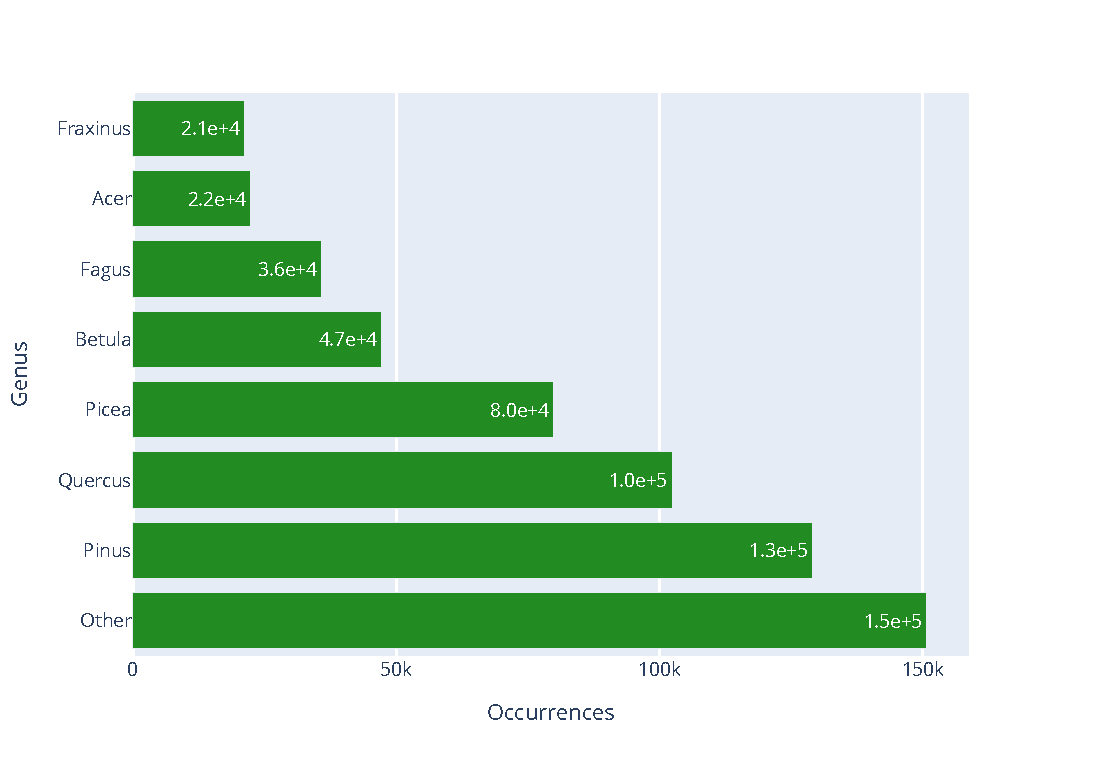
\includegraphics[width=0.48\linewidth, trim={0 0 2cm 0}]{figures/figures_labels/genus_cutoff.pdf}
    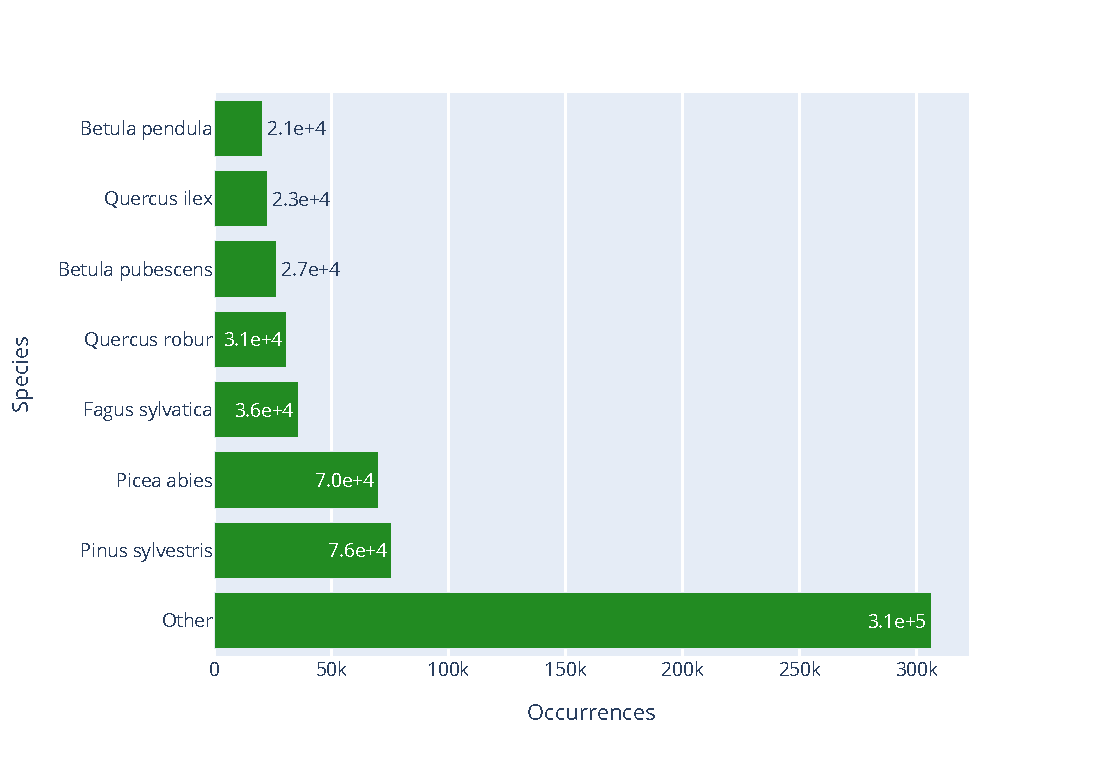
\includegraphics[width=0.48\linewidth, trim={0 0 2cm 0}]{figures/figures_labels/species_cutoff.pdf}

    \caption{Distribution of genera (left) and species (right) in EU-Forest.}
    \label{fig:cutoff_barplots}
\end{figure}

Integration with Sentinel-2 satellite data, which provides high-resolution multispectral images, allows for a robust model that leverages both ground-truth data and spectral information. The dataset, being relatively recent, offers a contemporary snapshot of forest conditions, ensuring that the trained model is relevant to current ecological and environmental conditions. 

The plots in Fig.\,\ref{fig:cutoff_barplots} underscore the prevalence of certain genera and species in European forests, providing valuable insights for training a CNN classifier. The dominance of specific genera and species in the dataset can enhance the classifier's ability to accurately identify and classify tree types when combined with Sentinel-2 data.

\begin{figure}[!thb]
    \centering

    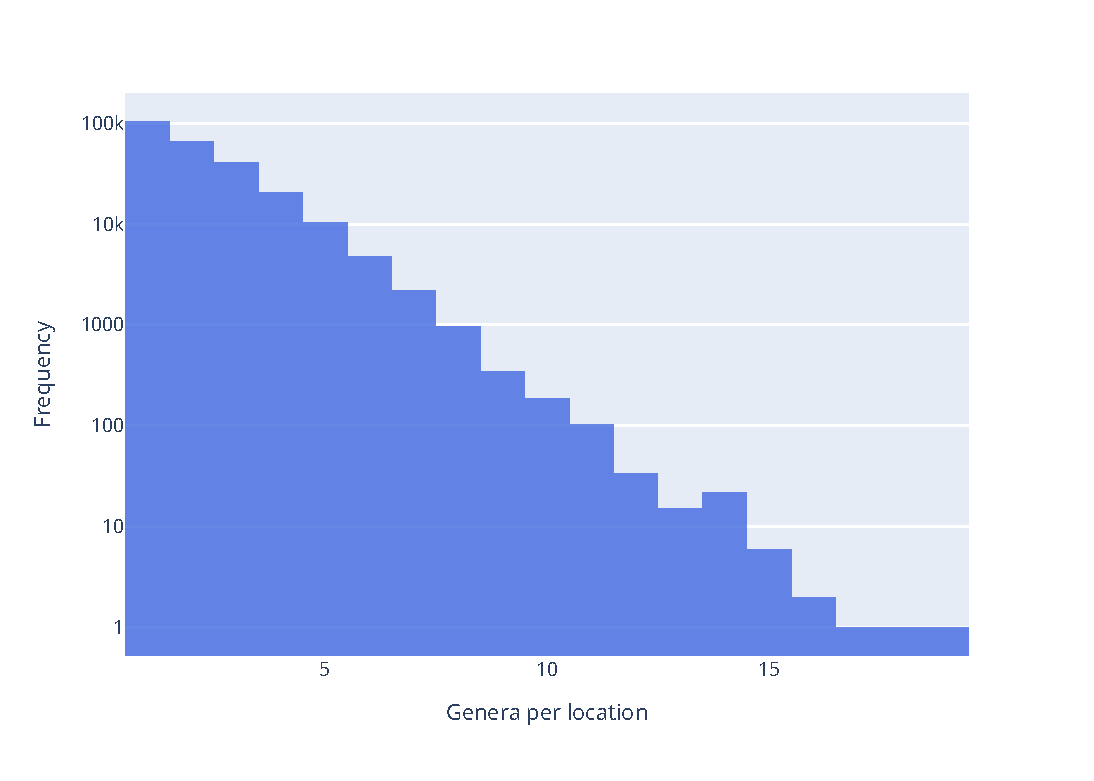
\includegraphics[width=0.48\linewidth, trim={0 0 2cm 0}]{figures/figures_labels/grouped_genus.pdf}%
    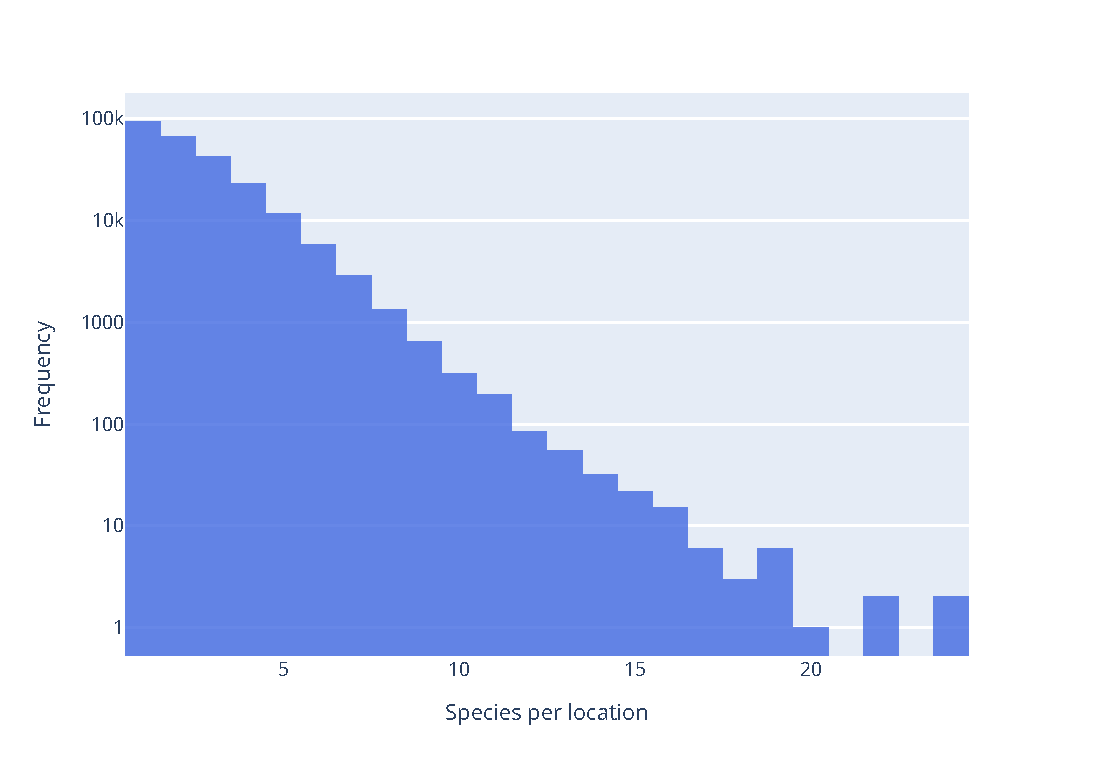
\includegraphics[width=0.48\linewidth, trim={0 0 2cm 0}]{figures/figures_labels/grouped_species.pdf}

    \caption{Distribution of genera (left) and species (right) per location.}
    \label{fig:grouped_histograms}
\end{figure}
 
The plots in Fig.\,\ref{fig:grouped_histograms} reveal a common pattern in biodiversity studies: most locations are characterized by a limited number of dominant genera and species, with a smaller number of locations exhibiting higher diversity. This pattern is important for training a CNN classifier, as it indicates that the classifier will often encounter locations with limited genera and species. However, it must also be capable of handling the less common, more diverse locations. The high-frequency, low-diversity areas will likely dominate the training process, influencing the classifier's ability to generalise across different forest types.

\section{Sentinel-2 Features}

\begin{figure}[ht]
    \centering
    \href{https://sentinels.copernicus.eu/documents/247904/4180891/Sentinel-2-infographic.pdf}
    {\includegraphics[width=0.9\linewidth]{figures/figures_sentinel/Sentinel-2-infographic.pdf}}
    \caption{Sentinel-2 mission infographic. It highlights important facts and achievements of the mission. Courtesy of \href{https://sentinels.copernicus.eu/web/sentinel/missions/sentinel-2}{ESA}.
    }
    \label{fig:sentinel2_info}
\end{figure}

Using Sentinel-2, Fig.\,\ref{fig:sentinel2_info}, specifically the 10-meter and 20-meter resolution bands, for training a CNN classifier of tree genera offers several significant advantages. Sentinel-2 provides high-resolution imagery with these bands capturing detailed spatial information essential for precise classification tasks.

The 10-meter resolution bands include visible red, green, and blue (RGB) wavelengths, as well as near-infrared (NIR) wavelengths, which are essential for assessing vegetation health and differentiating tree genera based on their reflectance properties. The 20-meter resolution bands encompass the red-edge, shortwave infrared (SWIR), and additional near-infrared regions, which enhance the classifier's ability to distinguish between tree genera by capturing subtle variations in spectral signatures. For subsequent analysis, the 20-meter bands were resampled to match the 10-meter resolution.

The multispectral imaging capability of Sentinel-2, with these selected bands, allows for detailed analysis and precise classification of tree genera. Each genus reflects and absorbs light differently across these wavelengths, providing rich data for the classifier to learn from and accurately identify tree types.

Moreover, Sentinel-2 has a frequent revisit time, with satellites passing over the same area every 5 days at the equator. This frequent update cycle is crucial for handling cloud cover, as it increases the likelihood of acquiring cloud-free images, ensuring that the classifier is trained on clear and usable data.

\begin{figure}[!thb]
    \centering

    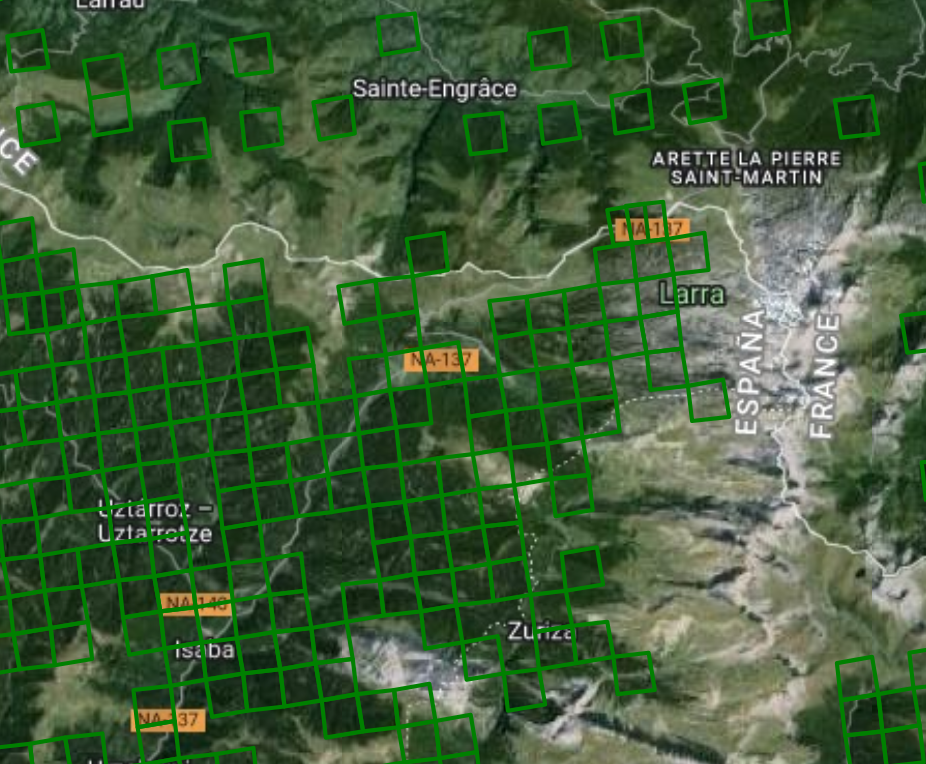
\includegraphics[width=0.48\linewidth]{figures/figures_sentinel/sample_area_earth.png}
    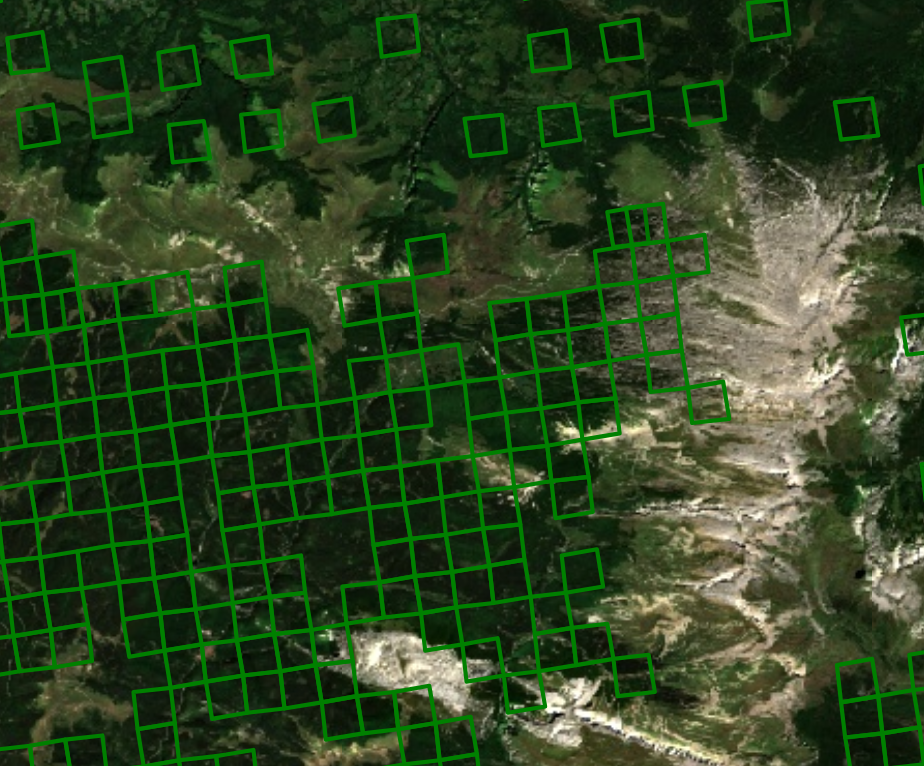
\includegraphics[width=0.48\linewidth]{figures/figures_sentinel/sample_area_sentinel.png}

    \caption{Multiple sample locations overlaid on Google Earth (left) and Sentinel-2 (right) images.}
    \label{fig:label_sample_area}
\end{figure}

Sentinel-2 also offers extensive geographical coverage, capturing large areas in each image. This comprehensive coverage is essential for training classifiers intended for wide-ranging applications across different forest types and regions, and it supports the development of global models for tree genus classification.

Additionally, Sentinel-2 data is freely available through the European Space Agency's Copernicus program and Google Earth Engine. This open access removes budget constraints, making high-quality satellite data accessible for various research and operational purposes.

\begin{figure}[!thb]
    \centering

    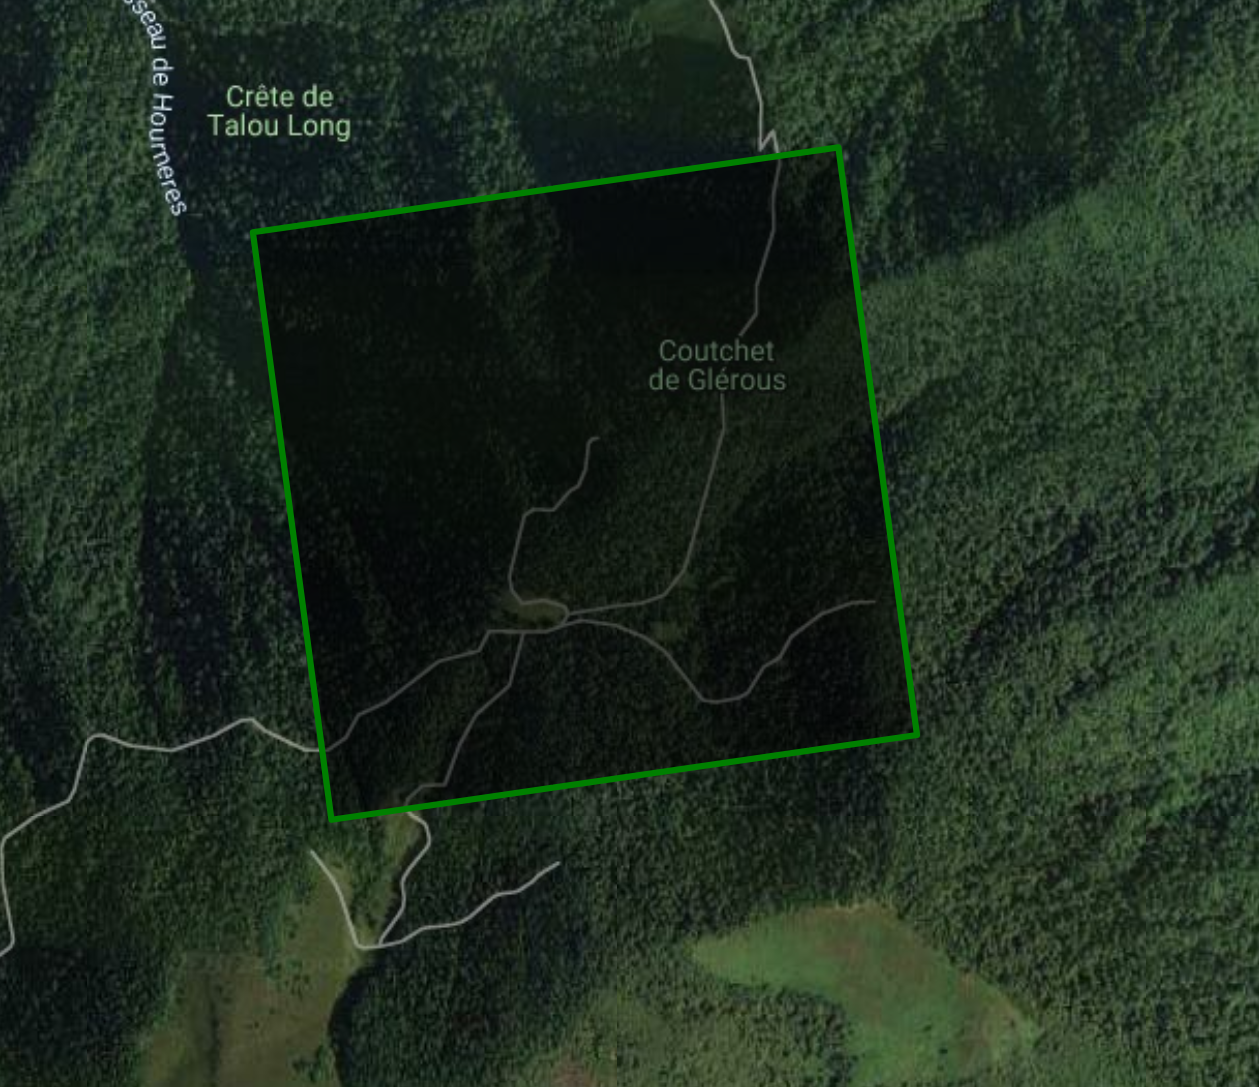
\includegraphics[width=0.48\linewidth]{figures/figures_sentinel/sample_earth.png}
    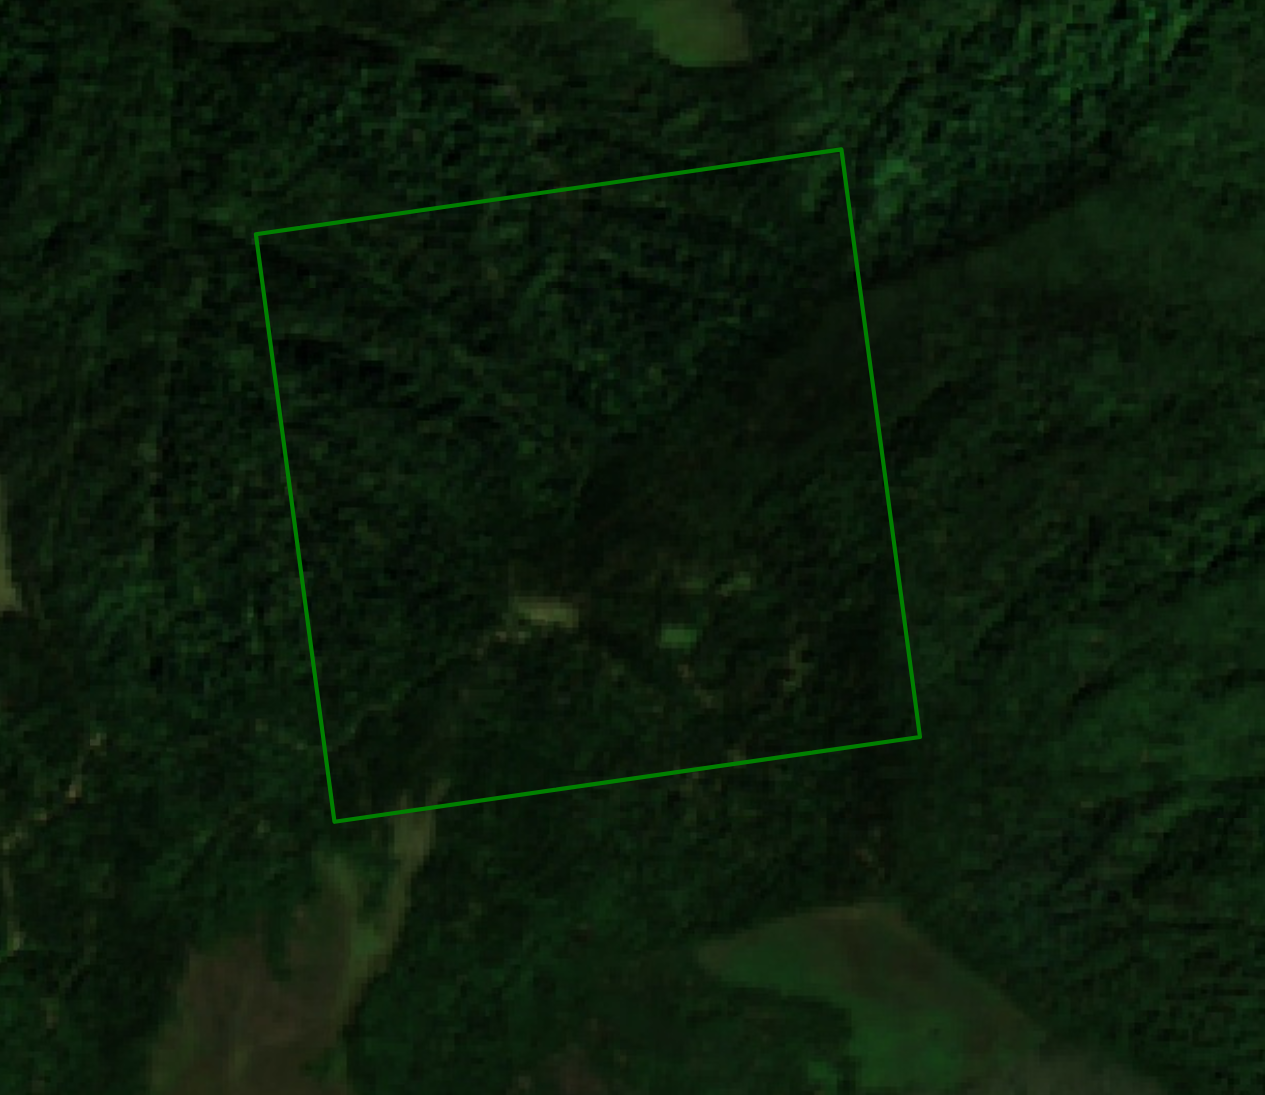
\includegraphics[width=0.48\linewidth]{figures/figures_sentinel/sample_sentinel.png}

    \caption{Sample location overlaid on Google Earth (left) and Sentinel-2 (right) images.}
    \label{fig:label_sample}
\end{figure}

Figs.\,\ref{fig:label_sample_area} and \ref{fig:label_sample} illustrate the integration of high-resolution geographical context with Sentinel-2 satellite data for detailed environmental analysis. The grid overlay in the images represents areas for data collection and analysis. The left images provide a more detailed geographical context, while the right images show how Sentinel-2 bands B2, B3, and B4 (blue, green, and red respectively) are structured and utilised for spectral analysis.


\begin{figure}[ht]
    \centering
    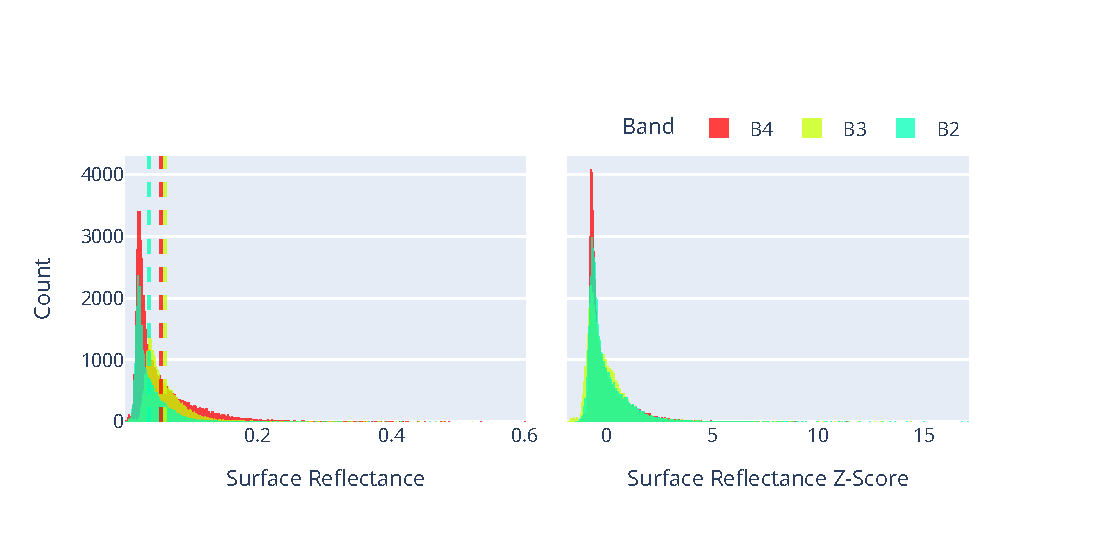
\includegraphics[width=0.98\linewidth, trim={15pt 25pt 10pt 50pt}, clip]{figures/figures_features/bgr_hist.pdf}
    \caption{Distributions for surface reflectance (left), including a sample means as a dotted line, 
    and z-score normalisation (right) for RGB.}
    \label{fig:bgr_hist}
\end{figure}

\begin{figure}[ht]
    \centering
    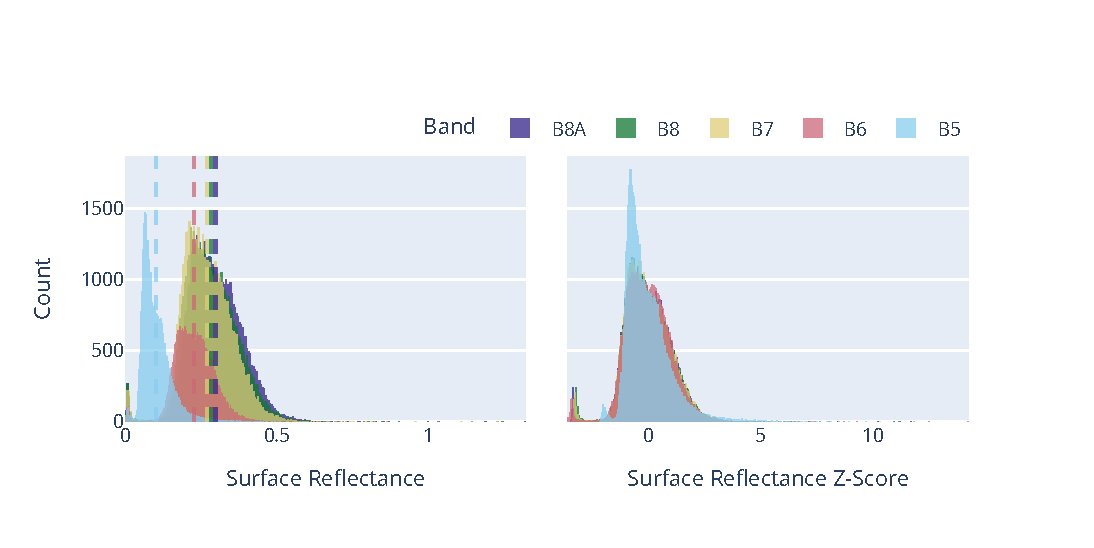
\includegraphics[width=0.98\linewidth, trim={15pt 25pt 10pt 50pt}, clip]{figures/figures_features/nir_hist.pdf}
    \caption{Distributions for surface reflectance (left), including a sample means as a dotted line, 
    and z-score normalisation (right) for NIR.}
    \label{fig:nir_hist}
\end{figure}

\begin{figure}[ht]
    \centering
    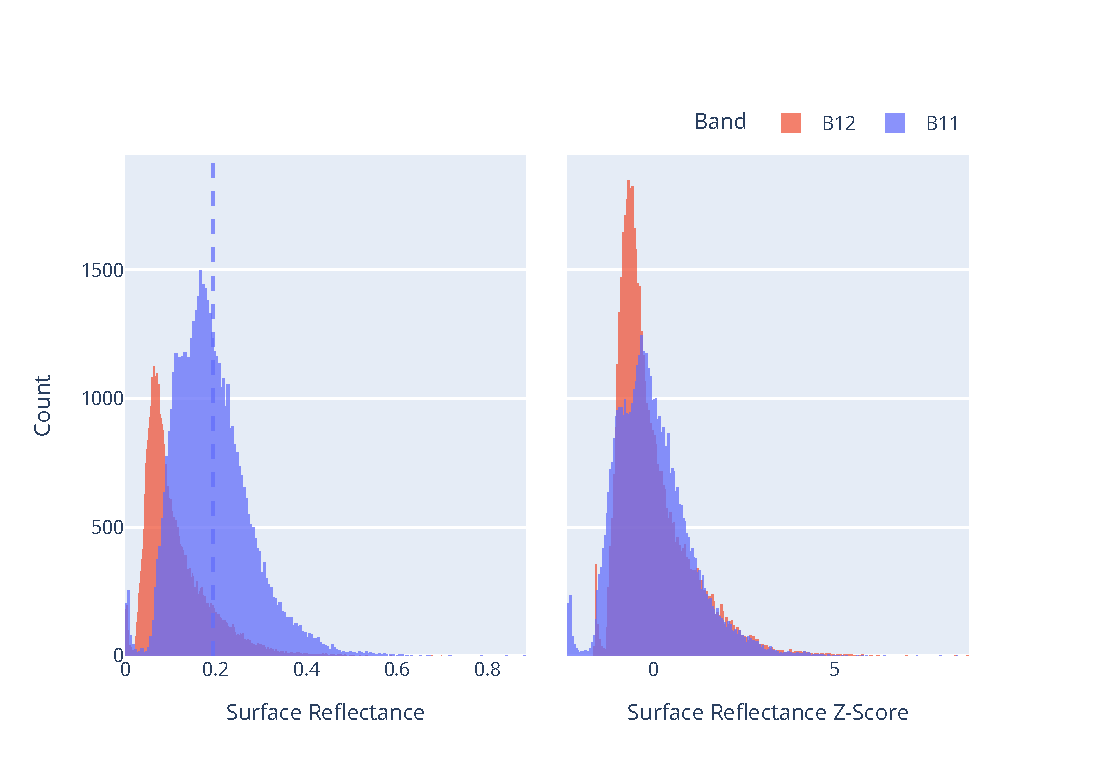
\includegraphics[width=0.98\linewidth, trim={15pt 25pt 10pt 50pt}, clip]{figures/figures_features/swir_hist.pdf}
    \caption{Distributions for surface reflectance (left), including a sample means as a dotted line, 
    and z-score normalisation (right) for SWIR.}
    \label{fig:swir_hist}
\end{figure}

Figs.\,\ref{fig:bgr_hist}, \ref{fig:nir_hist}, and\,\ref{fig:swir_hist} provide a detailed look at the distribution of surface reflectance values and their z-scores for various Sentinel-2 spectral bands, a normalisation method which is crucial for many classification tasks using CNNs. These figures use medians taken over the summer months (June, July, and August) between 2017, 2018, and 2019.

Fig.\,\ref{fig:bgr_hist} shows that the reflectance values for the bands B2, B3, and B4 generally follow a log-normal distribution. The z-scores for these bands peak near zero, demonstrating that the reflectance values have been normalized effectively. This normalisation is essential for ensuring that the values from different bands are on the same scale, which is particularly important when using CNN for classification.

Fig.\,\ref{fig:nir_hist} presents the distribution for the NIR bands B5, B6, B7, B8, and B8A. The reflectance values for these bands display a central tendency, with a significant number of pixels having values around the mean. The z-score distributions, peaking near zero, indicate successful normalisation of the reflectance values. Normalising the data in this way ensures that the CNN can process and compare these values more effectively, enhancing the model's ability to classify different types of tree genera accurately.

Fig.\,\ref{fig:swir_hist} shows histograms for the SWIR bands B11 and B12. The bands display a similar pattern, with the majority of reflectance values clustering on the left of the mean and tailing off to the right of the mean. The z-scores for these bands also peak at zero, confirming that the data has been normalised successfully. 


\begin{figure}[ht]
    \centering
    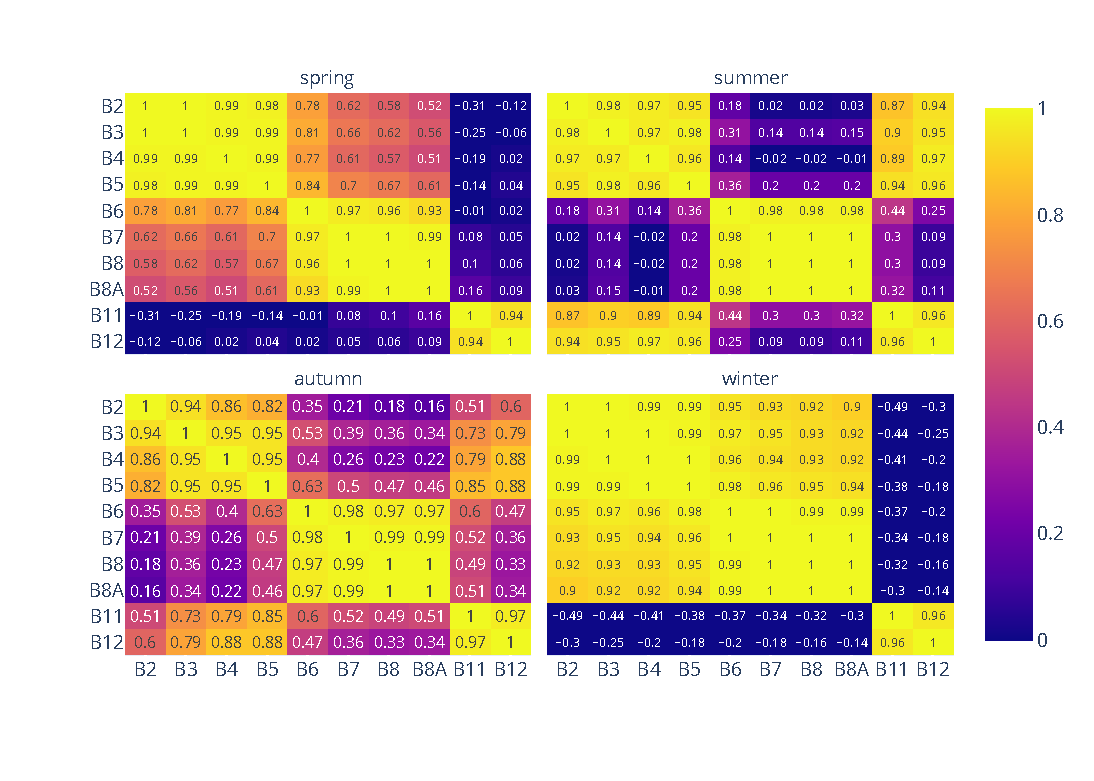
\includegraphics[width=0.9\linewidth, trim={40pt 40pt 10pt 30pt}, clip]{figures/figures_features/season_correlation.pdf}
    \caption{Seasonal Sentinel-2 band correlations.}
    \label{fig:season_correlation}
\end{figure}

The correlations among different spectral bands of Sentinel-2 data across seasons, as depicted in the correlation matrices in Fig.\,\ref{fig:season_correlation}, highlight significant patterns that are useful for tree genus classification. Each figure shows the correlation coefficients between various bands, providing insights into how these relationships change with the seasons.

During winter, all bands in NIR and RGB groups show very strong correlations with each other. These high correlations, often close to 1, indicate that the spectral responses of these bands are highly similar during this season. This consistency is likely due to the uniform reflectance properties of vegetation and the ground cover in winter. This strong correlation is beneficial for tree genus classification as it suggests that the data from these bands can be reliably used to distinguish tree genera based on their reflectance characteristics, or lack thereof, in winter.

In spring, the correlations remain high within the NIR and RGB groups but to a slightly lesser degree compared to winter. The correlation between these two groups starts to decrease, reflecting the changes in vegetation as new growth begins. This seasonal variation provides additional information that can be leveraged to improve the classification models, as the differences in reflectance between the bands become more pronounced.

During summer and autumn, while there are still strong correlations within the NIR and RGB groups, the correlation between these groups is notably lower. This reduced correlation can be attributed to the varying phenological stages of the trees, including differences in leaf development and moisture content. These seasonal changes affect the reflectance properties differently in the NIR and RGB bands. The distinct spectral responses during these seasons offer complementary information that can enhance the classification of tree genera by providing a more diverse set of data points that capture the variability in tree characteristics.

Overall, the varying correlations across seasons underscore the robustness of using Sentinel-2 data for tree genus classification. The normalisation of data using z-scores is crucial for bringing the values of different bands to the same scale, which is particularly important for CNNs. This normalisation ensures that the model can effectively process and compare the multi-band data, leading to more accurate classification results.

\section{Copernicus DEM GLO-30}

Integrating the Copernicus Global 30m Digital Elevation Model (DEM) data into the classification model can significantly enhance its performance for tree genus classification. Elevation data provides critical information about the terrain, which influences various ecological factors such as temperature, moisture availability, and soil type. These factors, in turn, affect vegetation types and distribution. By incorporating elevation data, the model can better understand the environmental context of each location, leading to more accurate predictions. For example, certain tree genera may be more prevalent at specific elevation ranges due to their adaptation to particular climatic conditions or soil properties. Therefore, integrating elevation data can help in distinguishing between tree genera that occupy different ecological niches.

Fig.\,\ref{fig:elevation_hist} presents the distribution of elevation values in meters, as well as the z-scores, which standardise these values. The elevation values range from 0 to around 2500 meters, with most data points clustered below 500 meters. This suggests that the majority of the study area is relatively low-lying. Standardising elevation values using z-scores is beneficial for integrating elevation data with spectral data, as it ensures that elevation values are on a comparable scale to the reflectance values from Sentinel-2 bands. 

\begin{figure}[ht]
    \centering
    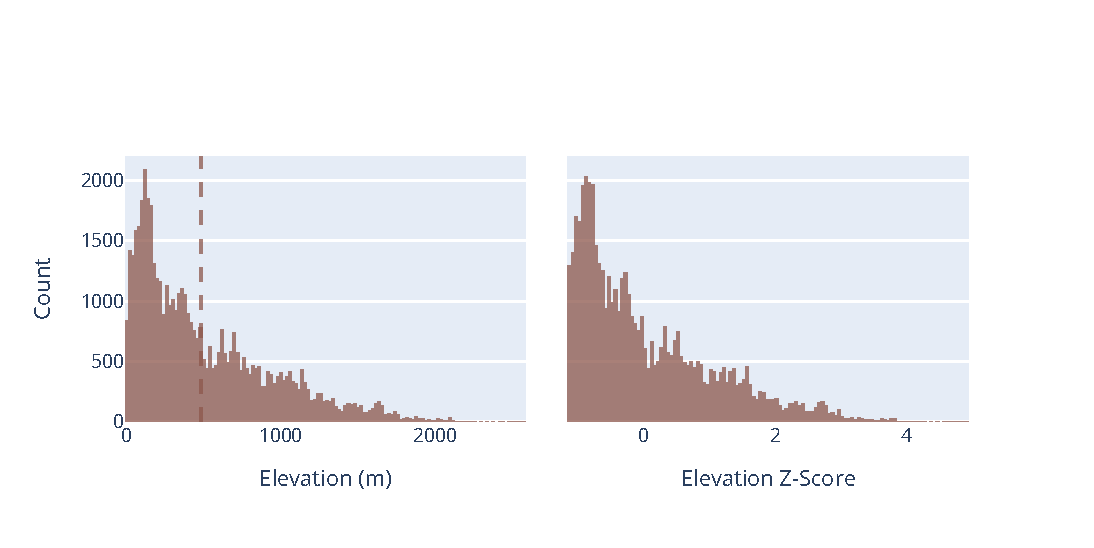
\includegraphics[width=0.98\linewidth, trim={15pt 25pt 10pt 50pt}, clip]{figures/figures_features/elevation_hist.pdf}
    \caption{Distributions for elevation (left), including a sample means as a dotted line, 
    and z-score normalisation (right) for the Copernicus DEM GLO-30 dataset.}
    \label{fig:elevation_hist}
\end{figure}

\section{SoilGrids}

The SoilGrids dataset (\cite{soil_report}) provides global soil information at a spatial resolution of 250 meters and incorporates quantified spatial uncertainty. It includes key soil properties such as organic carbon content, pH, sand, silt, and clay percentages, bulk density, cation exchange capacity, and more. These data are derived from machine learning models trained on extensive soil sample databases and environmental covariates.

Integrating SoilGrids data into the tree genus classification model can significantly enhance its performance. Soil properties profoundly influence vegetation types and distribution, as different tree genera have specific soil requirements and preferences. For instance, soil pH, nutrient content, and texture can determine the suitability of a habitat for particular tree species. By incorporating detailed soil composition data, the model can better understand the environmental context, leading to more accurate predictions of tree genera. This integration helps to account for the ecological niche of each genus, improving the robustness and precision of the classification.

\begin{figure}[ht]
    \centering
    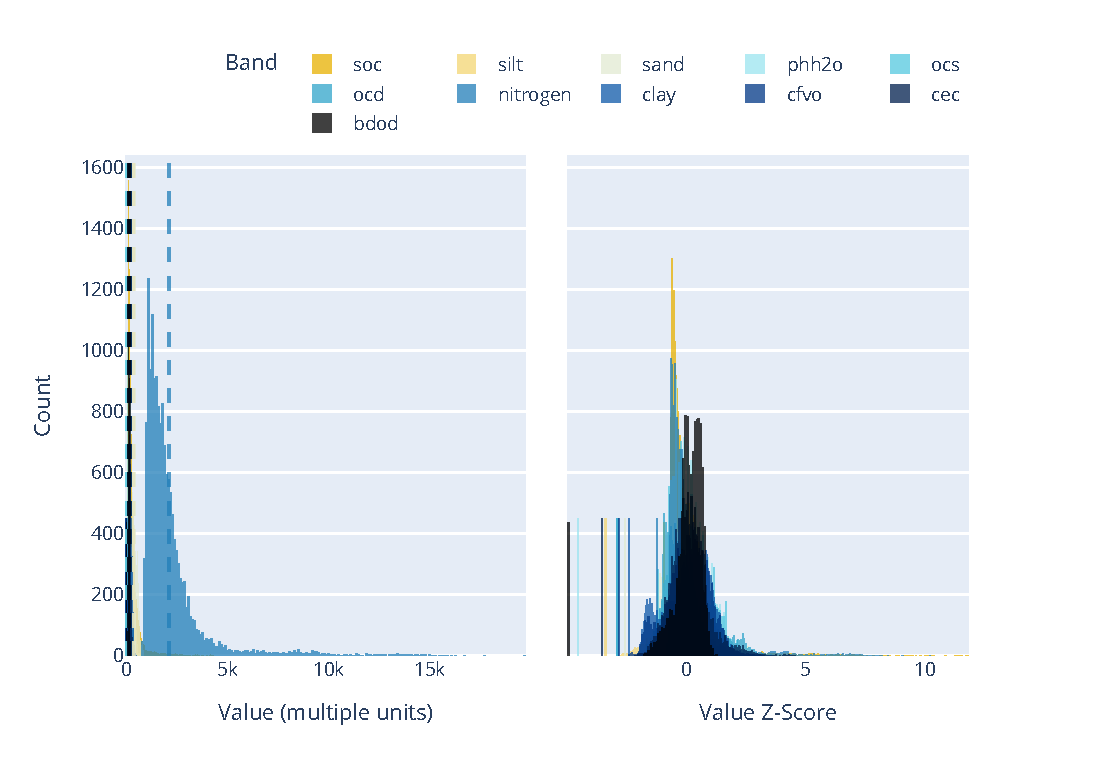
\includegraphics[width=0.98\linewidth, trim={15pt 25pt 10pt 20pt}, clip]{figures/figures_features/soil_hist.pdf}
    \caption{Distributions for elevation (left), including a sample means as a dotted line, 
    and z-score normalisation (right) for the Copernicus DEM GLO-30 dataset.}
    \label{fig:soil_hist}
\end{figure}

Fig.\,\ref{fig:soil_hist} displays the distribution of various soil properties present in the SoilGrids dataset. The x-axis represents the value of these properties in multiple units, while the y-axis represents the count of observations. Additionally, the z-score distribution is shown to standardise these values.

The distribution of soil properties varies, reflecting the diversity of soil types across the study area. The z-score distribution standardises these values, bringing them onto a common scale, which is essential for integrating soil data with spectral and elevation data in the classification model.
    \FloatBarrier
    \chapter{Feature Selection}
\label{chapter:analysis}

\section{Sentinel-2 Seasons}
\label{section:seasonal}

Fig.\,\ref{fig:seasonal_selection} shows the performance of the CNN model across different seasons, with metrics including recall, precision, weighted f1-score, precision-recall curve area under the curve (PRC), and receiver operating characteristic area under the curve (AUC). Filled boxes indicate the combination of seasons used to train and validate the model. Blue boxes indicate a combination of 3D CNN and fully-connected layers and the orange box indicates the use of a similar model but with the introduction Long Short-Term Memory (LSTM) alongside 3D convolutions and fully-connected layers.

\begin{figure}[ht]
    \centering
    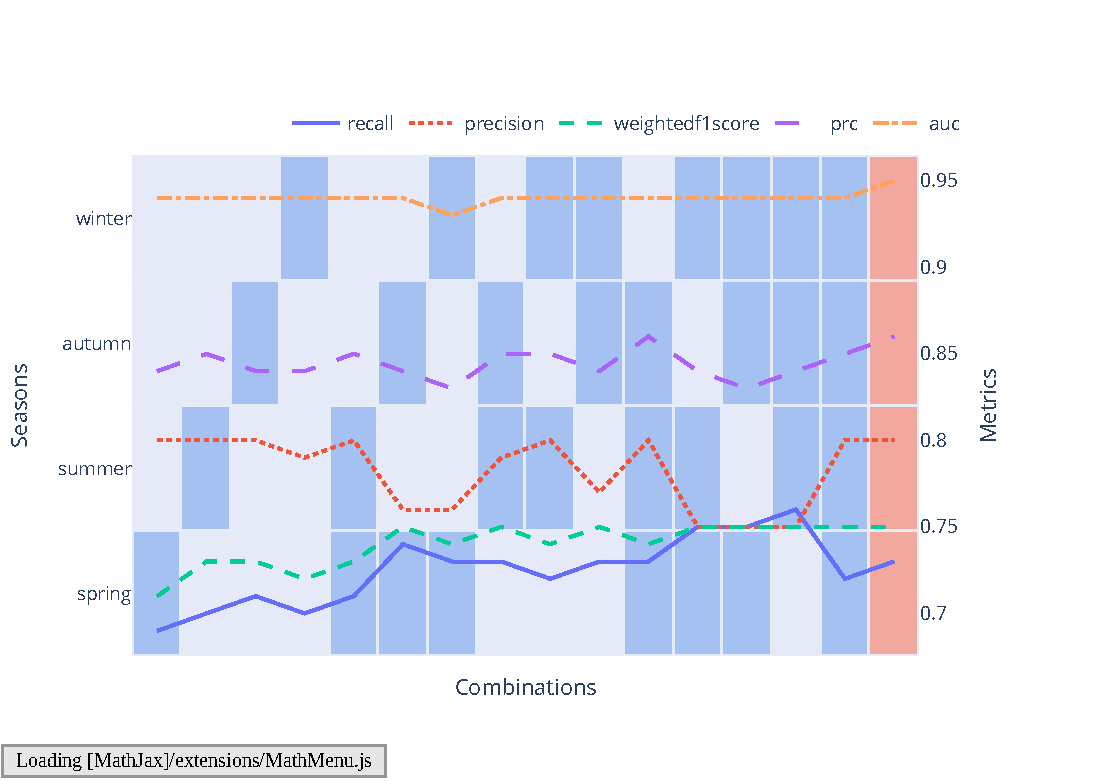
\includegraphics[width=0.9\linewidth, trim={20pt 40pt 10pt 30pt}, clip]{figures/figures_analysis/seasonal_selection.pdf}
    \caption{Seasonal Sentinel-2 analysis for all season combinations using a 3D CNN.}
    \label{fig:seasonal_selection}
\end{figure}

3D convolutions were selected for this model due to their suitability for this problem as they can effectively capture the spatial and spectral dependencies in the multi-temporal Sentinel-2 data. By considering the additional temporal dimension, 3D convolutions can leverage seasonal variations and changes in vegetation phenology, which are crucial for accurate tree genus classification.

LSTM was introduced to the model alongside 2D convolutions because they process the spatial structure of the Sentinel-2 images through convolution operations while simultaneously capturing temporal sequences. This dual capability allows the model to learn intricate spatial patterns within each image and understand how these patterns evolve over time.

The selected metrics used to create Fig.\,\ref{fig:seasonal_selection} are well-suited for handling class imbalance in the seasonal analysis of the CNN model. Recall ensures the model captures as many instances of the minority classes as possible, which is critical when dealing with imbalanced datasets. Precision assesses the accuracy of the model's positive predictions, reducing the impact of false positives. The weighted f1-score balances precision and recall, accounting for class imbalance by considering the support of each class. PRC focuses on the trade-off between precision and recall, highlighting the model's performance on minority classes. Lastly, AUC measures overall model performance across all thresholds, providing a comprehensive view of its ability to distinguish between classes.

For individual seasons, the model performs best in summer and autumn overall across the metrics. This suggests that the CNN model is more effective at classifying tree genera during these times, likely due to clearer and more distinct spectral signatures in the data collected during summer and autumn. The lower performance in spring and winter might be attributed to less distinct spectral signatures or more challenging environmental conditions, such as cloud cover and snow, which can affect data quality.

Based on the weighted f1-scores shown in Fig.\,\ref{fig:seasonal_selection}, adding more seasons does not seem to offer significant benefits. For instance, some two-season combinations, such as summer and autumn, performed on par with the more complex four-season models. Additionally, single-season models were only a few percentage points below the top-performing models.

Based on these results, further analysis focused solely on summer seasons. This approach benefits from faster model training and reduced storage requirements, as adding an extra season nearly doubles the storage needs, a challenge that intensifies with the extension of the analysis over additional years. Despite these adjustments, a complete Sentinel-2 dataset for a single season still requires nearly 200\,GB, or approximately 1\,MB per location.

\section{Sentinel-2 Bands}

\begin{figure}[ht]
    \centering
    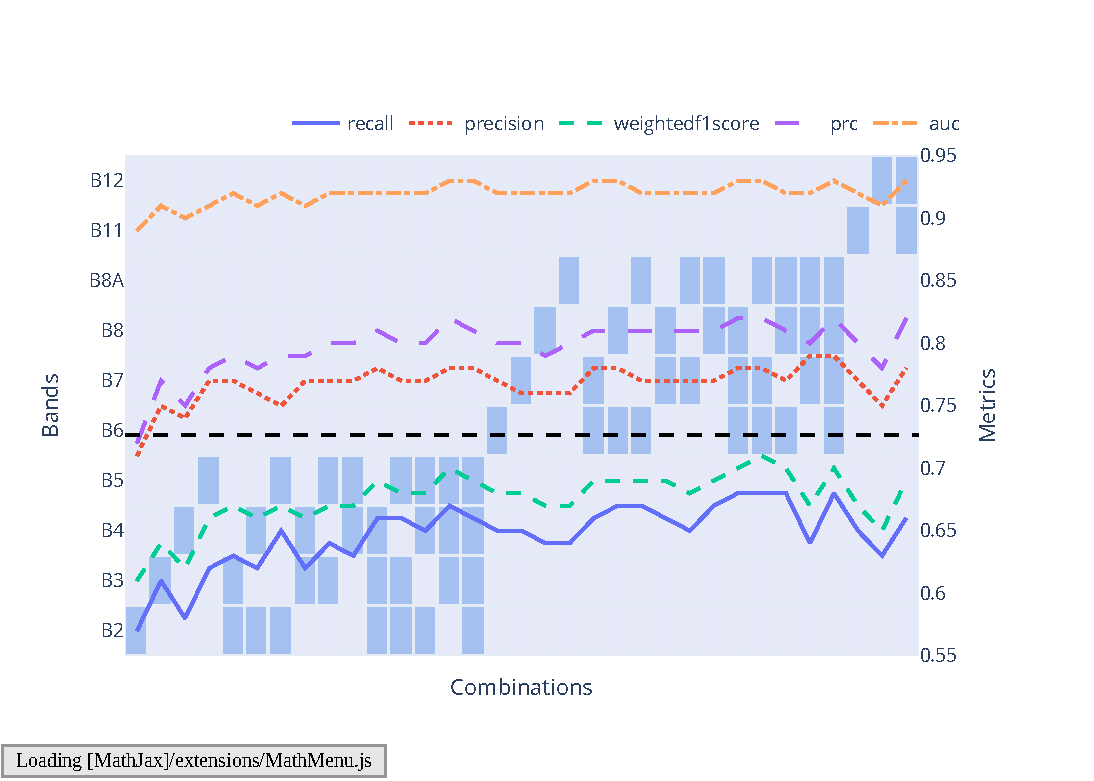
\includegraphics[width=0.9\linewidth, trim={20pt 40pt 10pt 30pt}, clip]{figures/figures_analysis/band_selection.pdf}
    \caption{Sentinel-2 analysis for all combinations within three band groups using a CNN. The horizontal black line represents the weighted f1-score for all bands.}
    \label{fig:band_selection}
\end{figure}

In addition to the seasonal analysis in Section\,\ref{section:seasonal}, another analysis was conducted to identify the most effective band combinations. Due to the large number of possible combinations, a direct analysis was impractical. Instead, Sentinel-2 bands were divided into three groups based on summer correlation groupings shown in Fig.\,\ref{fig:season_correlation}: B2, B3, B4, and B5; B6, B7, B8, and B8A; and B11 and B12. 

The resulting analysis, shown in Fig.\,\ref{fig:band_selection}, indicates that NIR and SWIR bands perform slightly better overall. Based on these results, another group was selected: B2, B3, B6, B8, and B11. These bands represented the best combinations that resulted in a practical analysis within the available timeframe.

\begin{figure}[ht]
    \centering
    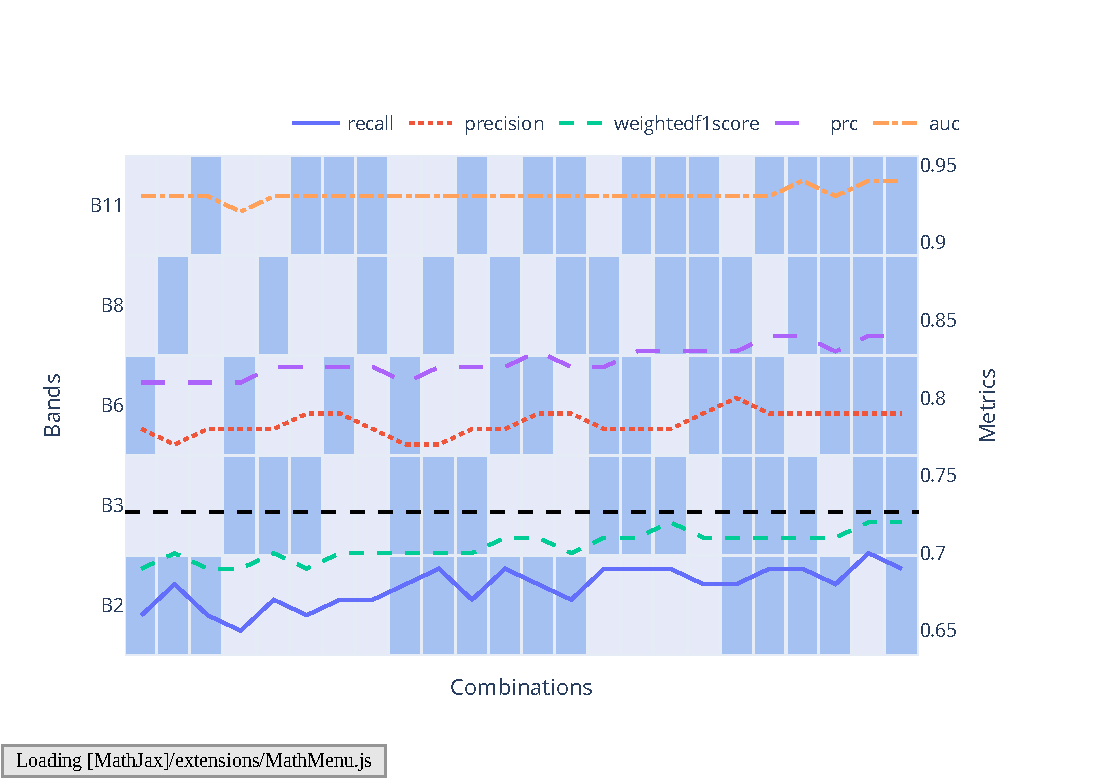
\includegraphics[width=0.9\linewidth, trim={20pt 40pt 10pt 30pt}, clip]{figures/figures_analysis/band_selection_further.pdf}
    \caption{Sentinel-2 analysis for selected combinations between each of the three groups using a CNN. The horizontal black line represents the weighted f1-score for all bands.}
    \label{fig:band_selection_further}
\end{figure}

Fig.\,\ref{fig:band_selection_further} shows that most selected combinations performed relatively well, as indicated by their proximity to the weighted f1-score for all bands. Based on these results, the most reasonable choices appear to be B3, B8, and B11, or the same but with B6 in addition. As the B6 combination displays better recall, precision, and weighted f1-score, as well as taking a fraction of storage compared to 10\,m bands due to being 20\,m. For the 250,000 samples, this combination should take roughly 50 GB of storage. As such, the combination B3, B6, B8, and B11, was used for the remainder of this study.

\section{Soil and Elevation}

\begin{figure}[ht]
    \centering
    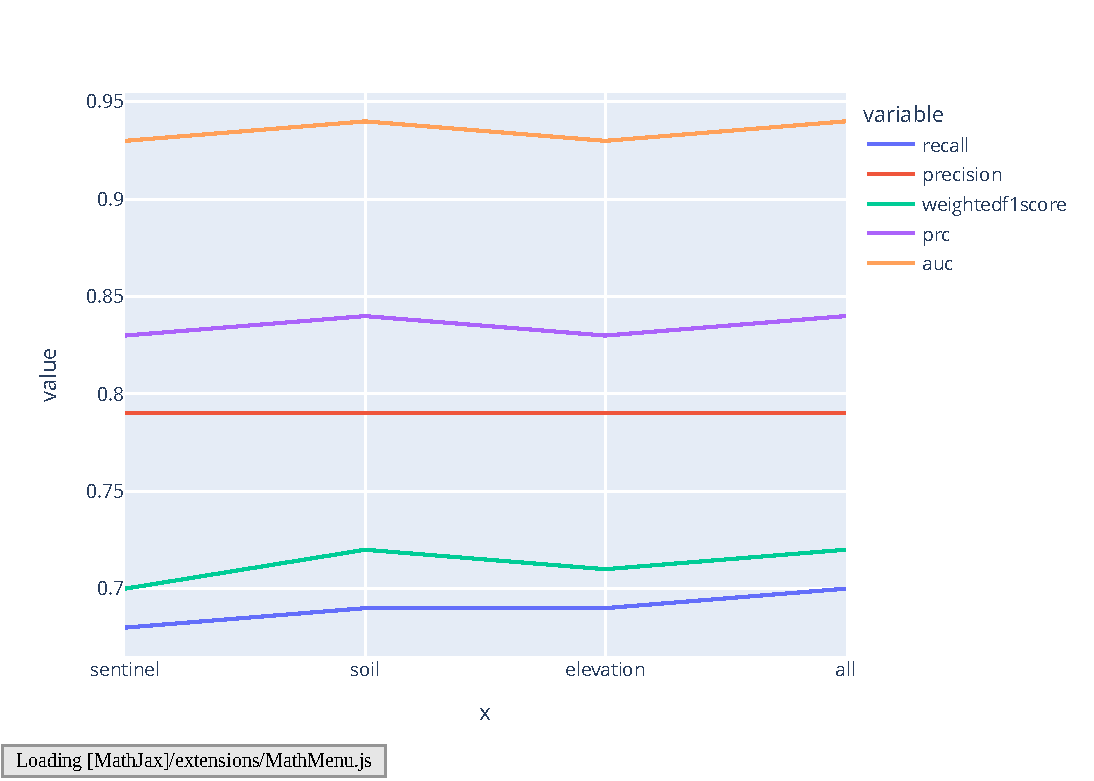
\includegraphics[width=0.9\linewidth, trim={20pt 40pt 10pt 30pt}, clip]{figures/figures_analysis/soil_elevation_analysis.pdf}
    \caption{Analysis of SoilGrids and elevation data integration.}
    \label{fig:soil_elevation_analysis}
\end{figure}

Fig.\,\ref{fig:soil_elevation_analysis} demonstrates the performance metrics for different combinations of Sentinel-2, SoilGrids, and elevation data in tree genus classification. Sentinel-2 data alone provides a solid baseline, attributed to its high resolution and rich spectral information. When considering SoilGrids data alone, the metrics are lower than those for Sentinel-2, reflecting the coarse resolution and potentially limited predictive power for this specific task. Similarly, elevation data alone shows lower performance metrics, indicating that while elevation is a relevant feature, it does not provide sufficient information by itself for accurate classification of tree genera. The combined use of these datasets shows marginal improvements, suggesting that while additional data may contribute some value, Sentinel-2's high-resolution spectral data is the most significant factor in the model's performance.

Given that Sentinel-2 data alone provides strong results, further enhancements and optimizations were solely focused on this dataset. 

\section{Summary}
    \FloatBarrier
    \chapter{Neural Network Configuration}
\label{chapter:hyper}
\section{Hyperparameter Optimization}

\begin{table}
\caption{Summary of initial hyperparameter search space.}
\label{tab:fixed_layers}
\begin{tabular}{ll}
\toprule
name & values \\
\midrule
class\_weight & [true, false] \\
training\_years & ['2017\_2018\_2019', '2017'] \\
kernel\_regularizer & ['l1l2', 'l1', 'l2'] \\
spatial\_dropout & [0.3, 0.1, 0.5] \\
activation & ['leaky\_relu', 'relu'] \\
pool\_size & [4, 2] \\
dropout & [0.3, 0.1, 0.5] \\
bias\_initializer & [true, false] \\
learning\_rate & [0.001, 0.0001, 0.01] \\
loss\_function & ['binary\_focal\_crossentropy', 'binary\_crossentropy'] \\
\bottomrule
\end{tabular}
\end{table}



Table\,\ref{tab:fixed_layers} provides a summary of the search space for the initial hyperparameter tuning process. These parameters are critical as they influence the model's learning process, generalization ability, and susceptibility to issues such as overfitting or bias. The chosen values in the search space represent a balance between exploring a wide range of options and focusing on promising areas based on prior knowledge or domain-specific considerations.

\begin{figure}[ht]
    \centering
    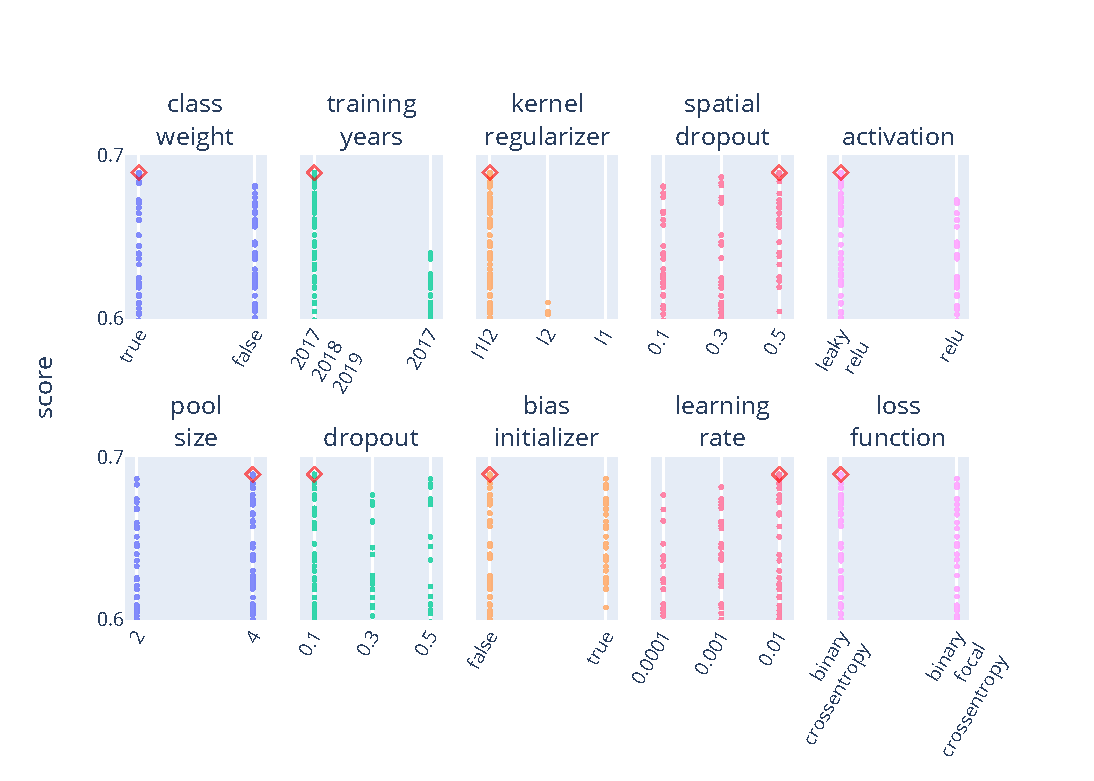
\includegraphics[width=0.9\linewidth, trim={10pt 10pt 40pt 40pt}, clip]{figures/figures_tuner/fixed_layers.pdf}
    \caption{The top f2-scores for the initial hyperparameter tuning process are highlighted, with the best score marked by a diamond shape.}
    \label{fig:fixed_layers}
\end{figure}

In the most successful trial, the model utilized training data from the medians of 2017, 2018, and 2019, applied L1L2 kernel regularization, used a spatial dropout rate of 0.5, and employed Leaky ReLU activation. The pool size was set to 4, dropout to 0.1, and bias initialization was disabled. The learning rate was 0.01, and the loss function was binary crossentropy, resulting in a score of 0.69.

While some of the initial trial's hyperparameters do not show significant overall improvement, some parameters do stand out. This is illustrated in Fig.\,\ref{fig:fixed_layers}, particularly regarding training years, kernel regularization, activation function, and learning rate.

\section{Model Architecture}

\begin{figure}[ht]
    \centering
    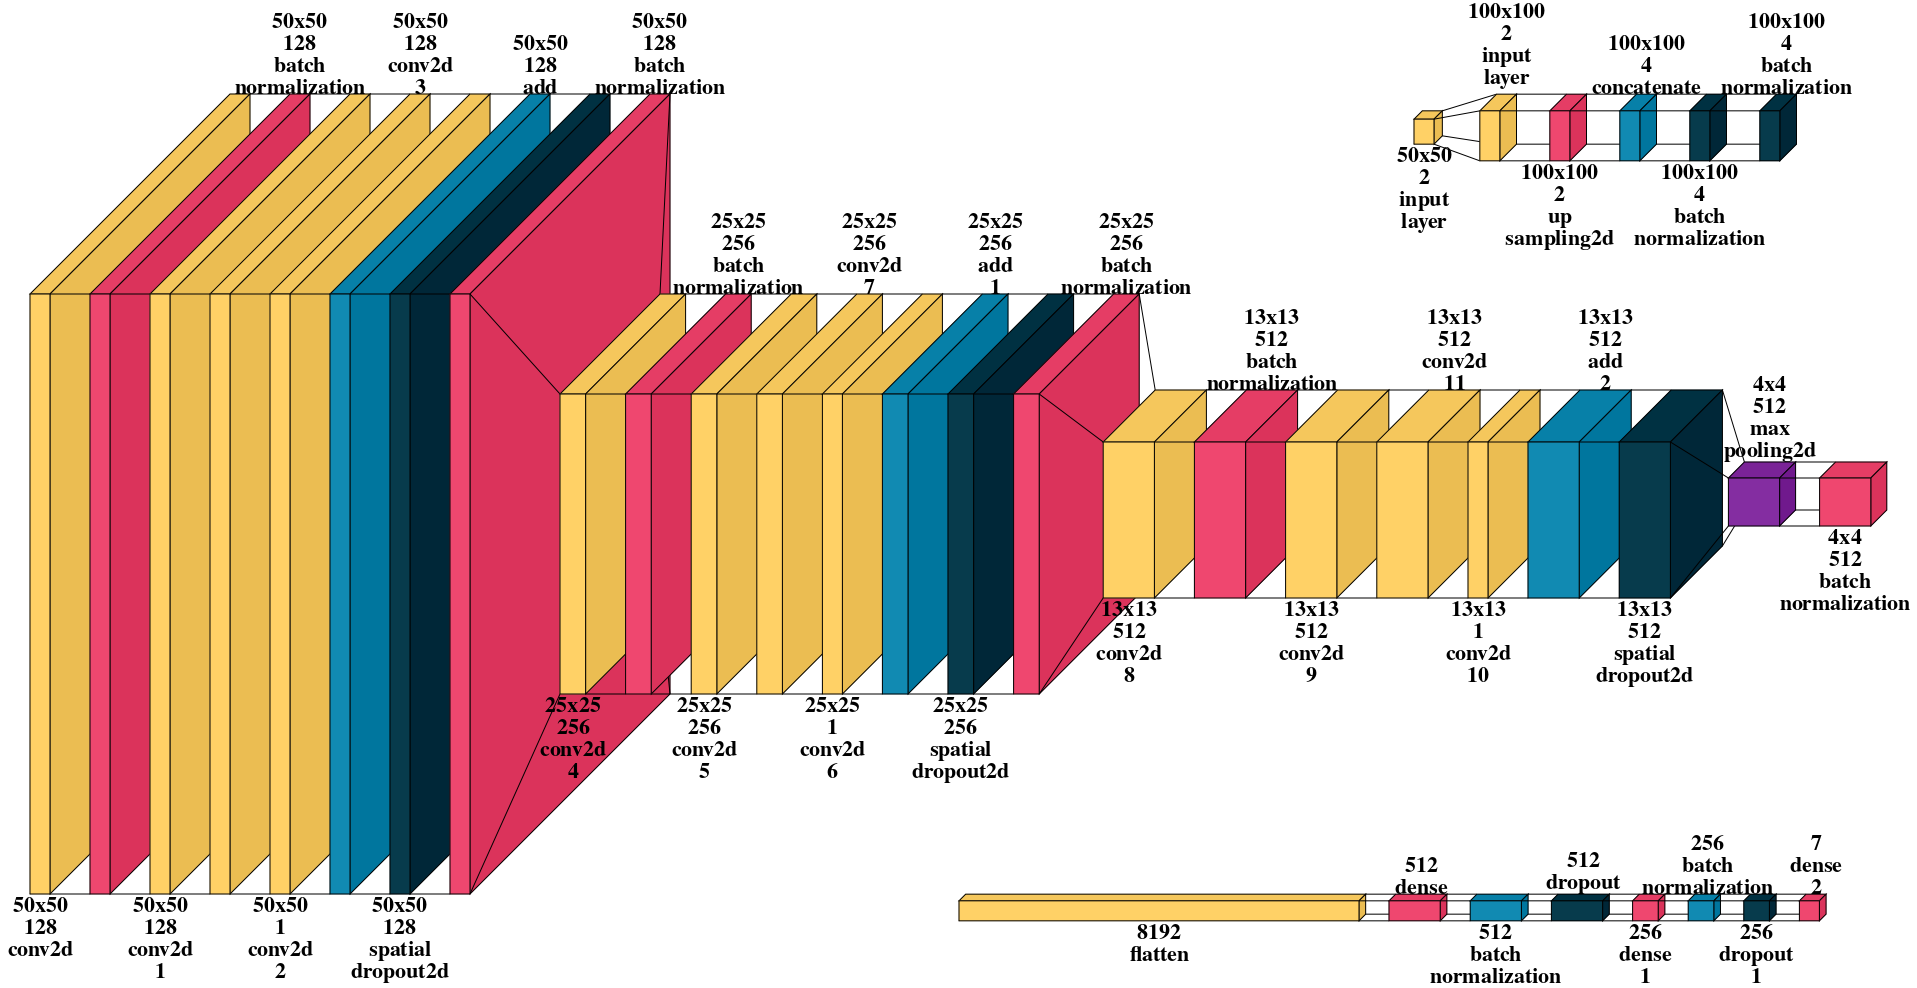
\includegraphics[width=0.9\linewidth]{figures/figures_tuner/model_layered_view.png}
    \caption{The model's layered architecture is depicted. The top-right shows the input layers, the middle section displays the convolutional layers, and the bottom-right illustrates the fully-connected layers. The layered views were generated using VisualKeras (\cite{visualkeras}).}
    \label{fig:model_layered_view}
\end{figure}

Fig.\,\ref{fig:model_layered_view} illustrates the detailed architecture of the deep learning model, highlighting the flow of data through its various layers. The model starts with input layers, which include upsampling layers to handle inputs with different dimensions. This ensures that all input sources are properly aligned for processing within the model. The network then progresses through multiple convolutional layers, with filter sizes generally increasing as the layers deepen. Batch normalization and dropout layers are strategically placed to regularize the model and prevent overfitting.

The architecture incorporates residual connections, which are crucial for maintaining gradient flow during backpropagation. These connections enable the network to be deep without suffering from issues like vanishing gradients, as highlighted in \cite{resnet}. As the network advances, spatial dimensions are reduced through pooling and striding operations, leading to a flattening layer that prepares the data for the fully connected (dense) layers. These dense layers further reduce the dimensionality, eventually outputting a 7-dimensional vector corresponding to the classification into 7 different tree genera, aligning with the model's goal of predicting tree types.


    \FloatBarrier
    \chapter{Climate Data}
\label{chapter:climate}
\section{ERA5 Dataset}

The ECMWF Reanalysis v5 (ERA5) dataset (\cite{era5}) was selected for correlating with tree genus classification due to its extensive and high-resolution climate data, which includes variables such as temperature, precipitation, and soil moisture. This dataset offers detailed historical weather information, capturing both spatial and temporal variations essential for understanding the environmental conditions that impact tree growth and distribution. By leveraging ERA5 data, this study aimed to explore how different climate factors might influence the abundance of various tree genera.

\begin{figure}[ht]
    \centering
    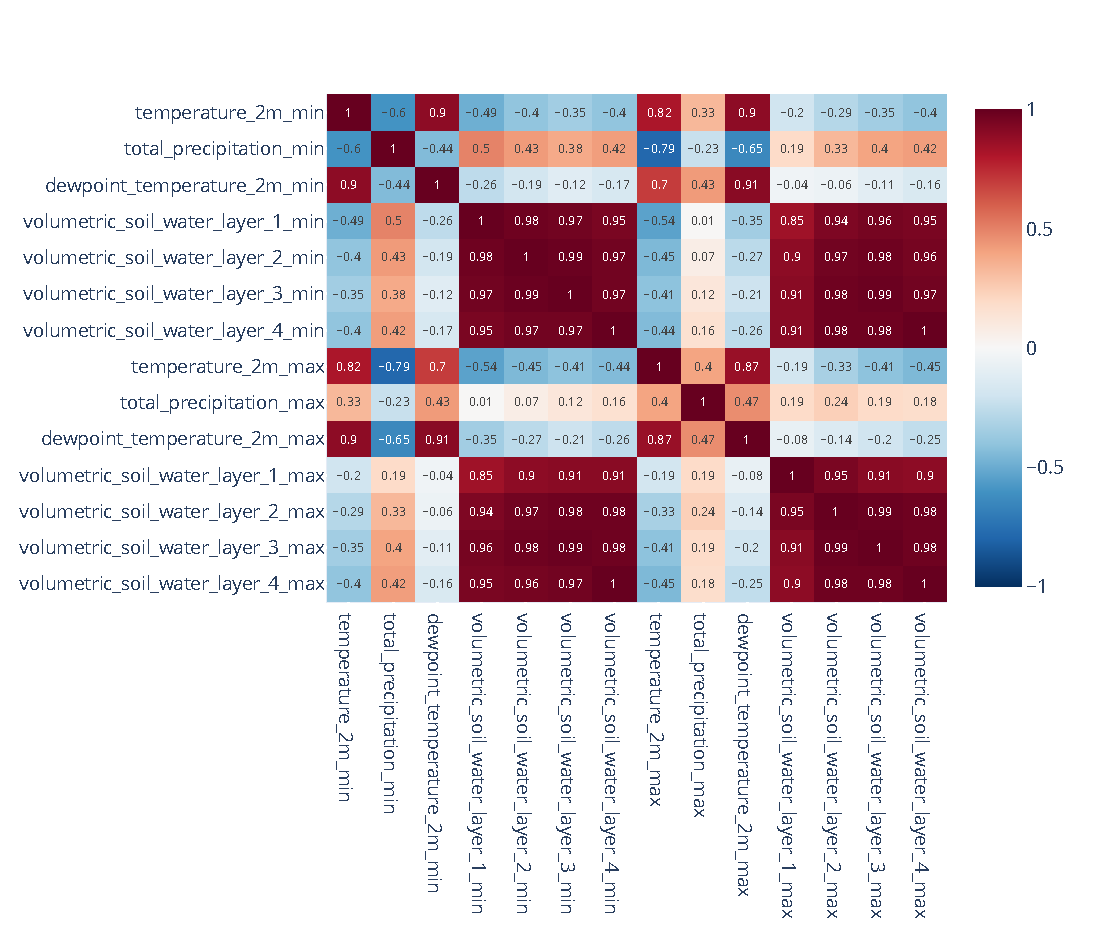
\includegraphics[width=0.96\linewidth, trim={20pt 20pt 10pt 40pt}, clip]{figures/figures_climate/weather_correlations.pdf}
    \caption{Correlations heatmap between various ERA5 variables. The data was downloaded from \cite{era5_dataset}, where detailed information is available.}
    \label{fig:weather_correlations}
\end{figure}

\section{ERA5 Exploration}

As the ERA5 dataset contains numerous meteorological variables, a selection was made based on domain knowledge, correlations (Fig.\,\ref{fig:weather_correlations}), and studies such as \cite{climate_choice}. Fig.\,\ref{fig:selected_variables_stats} summarizes this selection, showing the median and quantiles for the aggregated dataset across all study locations. The figure illustrates the significant variability within Europe, with the top-left plot indicating a difference of approximately 50\,K between the 1.0 quantile of minimum and maximum temperature measurements. This suggests that, although limited to Europe, this study explored a significant climate gradient. 

\begin{figure}[ht]
    \centering
    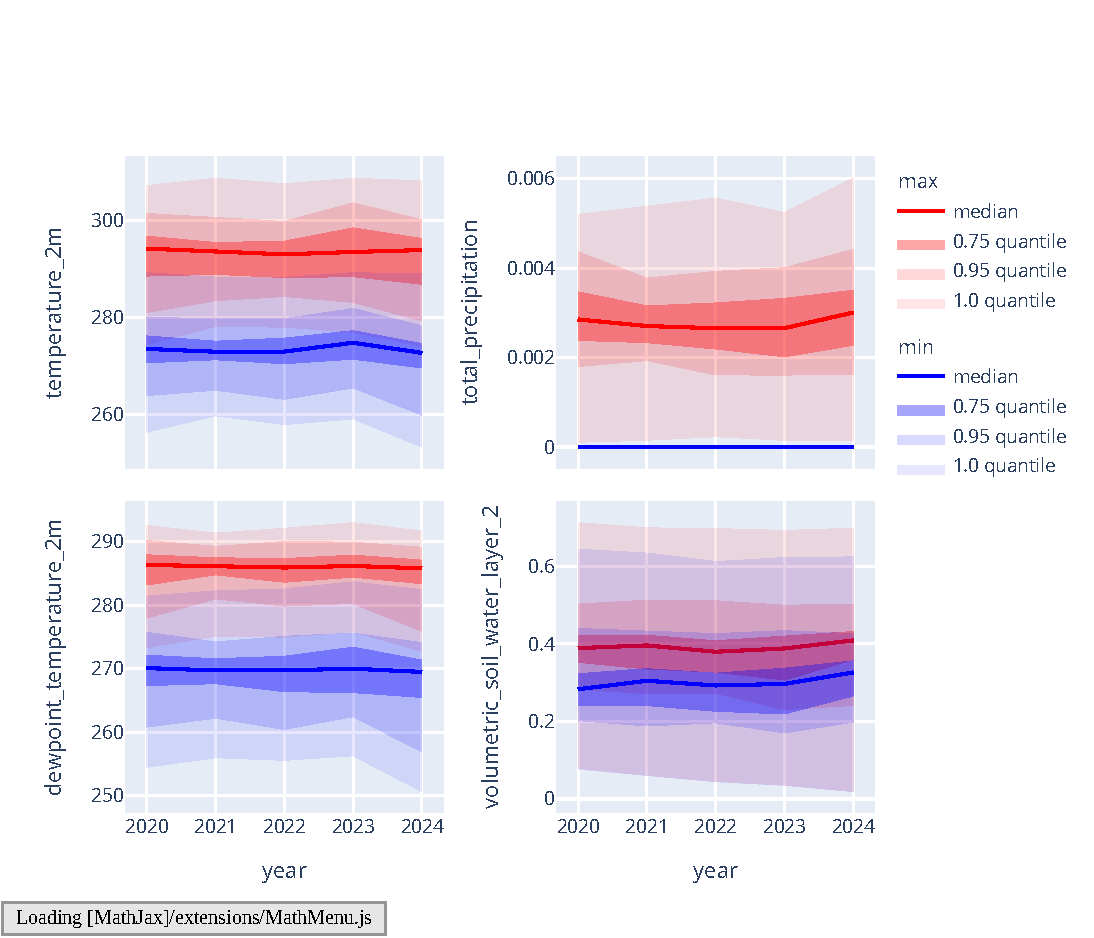
\includegraphics[width=0.98\linewidth, trim={20pt 20pt 10pt 40pt}, clip]{figures/figures_climate/selected_variables_stats.pdf}
    \caption{Median and quantiles of various monthly ERA5 variables by year.}
    \label{fig:selected_variables_stats}
\end{figure}

    \FloatBarrier
    % \chapter{Introduction}
\label{chapter:intro}

Forests play a critical role in regulating the Earth's climate and supporting biodiversity, as emphasized by studies such as \cite{bonan2008forests} and \cite{watson2018intact}. However, they are increasingly threatened by human activities and environmental changes, including deforestation, land-use conversion, and climate change, which are well-documented in \cite{fao2020gfra} and \cite{hansen2013forestcover}. Understanding the composition and dynamics of forest ecosystems is essential for effective conservation and management efforts, as discussed in \cite{turner2003remotesensing}. Accurate mapping of tree species and monitoring changes in forest cover over time, as demonstrated by \cite{sexton2013treecover}, are fundamental tasks in ecosystem management. Such maps provide valuable information for assessing biodiversity, tracking habitat loss, and understanding the impacts of climate change on forest ecosystems, as detailed by \cite{vose2018forests}.

\section{Remote Sensing and Machine Learning in Forest Monitoring}

Remote sensing technologies, including satellite imagery and LiDAR data, have revolutionized the ability to map and monitor forests at regional and global scales. Satellite imagery has provided comprehensive coverage and frequent updates, while LiDAR data offers precise measurements of forest structure, as shown in \cite{pettorelli2016satellite} and \cite{lefsky2002lidar}. Recent advancements in machine learning algorithms, particularly Convolutional Neural Networks (CNNs) and Random Forests (RF), have significantly enhanced the accuracy of tree species predictions from remotely sensed data (\cite{zheng2019deep, breiman2001random}). This study aims to develop and evaluate methods for generating tree genus predictions and change maps using these advanced remote sensing technologies. By leveraging these innovations, this study aims to advance our understanding of forest responses to environmental changes. Building on the methodologies and findings of recent studies such as \cite{hansen2013forestcover}, \cite{belgium_classification}, \cite{pakistan}, \cite{copernicus_main}, and \cite{germany_bavaria}, this research seeks to refine and enhance predictive models and change maps, offering new insights into how forests adapt to and are affected by shifting environmental conditions.

\section{Data Integration and Methodology}

In this research, high-resolution Sentinel-2 imagery has been integrated with detailed EU-Forest data (\cite{eu_forest_data}), Copernicus DEM elevation information (\cite{dem_dataset}), SoilGrids soil properties (\cite{soil_report}), and ECMWF Reanalysis v5 (ERA5) climate data (\cite{era5_dataset}). This combination of datasets provides a robust foundation for developing a CNN classifier. The classifier is designed to accurately identify tree genera across diverse European landscapes. Sentinel-2 imagery provides detailed multispectral data at a 10-meter and 20-meter resolutions, capturing the intricate spectral signatures of vegetation. The EU-Forest dataset offers essential ground-truth data across about 250,000 locations in Europe, facilitating the training and validation of machine learning models. Elevation data from the Copernicus DEM GLO-30 dataset introduces topographical context that influences vegetation distribution, while SoilGrids provides comprehensive soil composition information crucial for understanding the ecological niches of various tree genera.

Furthermore, climate variables, including temperature, precipitation, and soil moisture, have been integrated into the analysis to model the relationships between environmental factors and vegetation dynamics. This integration aims to provide deeper insights into how climate change is affecting forest ecosystems and to enhance the predictive power of the classification models. By combining these diverse datasets, the study endeavors to create a more nuanced and reliable model for tree genus classification.

\section{Challenges and Considerations}

Detecting changes in forest composition is essential for assessing the impacts of disturbances such as wildfire, climate change, and tree diseases. Time-series analysis of satellite imagery, combined with advanced algorithms for change detection, can enable researchers to quantify forest dynamics and identify areas undergoing significant ecological transitions. The inclusion of climate data further enriches this analysis by allowing for the exploration of how shifting environmental conditions are influencing forest ecosystems over time.

Despite these efforts, several challenges persist in remote sensing-based tree species or genus classification and change mapping. These include the need for improved methods to handle the complexity of forest ecosystems, increasing the availability of ground-truth data, incorporating uncertainty into mapping algorithms, and scaling up analyses to cover larger geographical areas. Additionally, the addition of elevation, soil, and climate data in this study resulted in only marginal improvements in model accuracy, prompting a critical evaluation of the relative importance of spectral versus environmental data in tree genus classification. This outcome suggests that while these additional datasets provide valuable context, their practical impact on classification accuracy within this specific framework may be limited.

This research highlights the complexities and trade-offs involved in integrating multi-source data into remote sensing models for forest monitoring. The findings underscore the importance of continued exploration and refinement of methodologies to optimize the use of diverse environmental datasets in understanding and conserving forest ecosystems in the face of global environmental change.

\section{Tools and Software}

The analysis was conducted using a combination of Python files and Jupyter notebooks. Data for the study was obtained through the Google Earth Engine Python API. The pre-processing of this data involved several libraries, including NumPy, Scikit-Learn, Pandas, and GeoPandas. Data visualization was carried out using Plotly, Geemap, and Holoviews. For model development, TensorFlow and Keras were utilized to build and train machine learning models. Hyperparameter tuning was performed with Keras Tuner and the Hyperband algorithm to enhance model performance. The code created for this study can be found at \url{https://github.com/pj097/ClimateForestModeling}.
    % \chapter{Research Framework}
\label{chapter:frame}
\section{Research Question}

Can we generate tree species predictions and change maps using remote sensing data and existing ground-truth data to assist in mitigating the impacts of climate change on forest ecosystems?

\section{Justification}

Forests are vital for maintaining biodiversity, regulating the climate, and providing essential ecosystem services. However, they are increasingly vulnerable to the effects of climate change, including shifts in temperature and precipitation patterns, increased frequency and intensity of extreme weather events, and altered disturbance regimes. Understanding how forests are responding to these changes is crucial for effective conservation and management efforts.

By developing methods to generate tree species predictions and change maps from remote sensing data, this research will attempt to address a pressing need for tools to monitor and assess the impacts of climate change on forest ecosystems. Such maps can provide valuable insights into changes in species composition, distribution, and health over time, helping to identify areas of conservation concern, prioritise management interventions, and inform climate adaptation strategies.

\section{Research Objectives}

\begin{itemize}
\item Establish accurate prediction models using remote sensing data and ground-truth labels.
\item Identify changes in forest cover over time, contingent on the success of the tree species prediction models.
\item Analyse the influence of climate variables on forest dynamics, depending on the quality of tree species predictions and change detection results.
\item Summarise findings and propose further research or practical applications.
\end{itemize}

\section{Measurement of Achievements}

\begin{itemize}
\item Evaluate the accuracy and reliability of tree species prediction and change detection algorithms.
\item Assess the ability to effectively integrate climate data and analyse its influence on forest dynamics, conditional on the quality of initial results.
\item Determine how useful the generated maps are for informing conservation and management decisions.
\item Suggest next steps and areas for further investigation based on the study's findings.
\end{itemize}


    % \chapter{Methodology}

\section{Develop Methods for Tree Species Predictions}

\begin{itemize}
  \item \textbf{Data collection:} gather multi-temporal, multi-spectral satellite imagery covering the study area. Obtain ground-truth data on tree species composition through existing forest inventory datasets.

  \item \textbf{Data exploration:} visualise the data and use statistical techniques to describe dataset characterisations, such as size, quantity, and accuracy, in order to better understand the nature of the data.
  
  \item \textbf{Pre-processing:} pre-process the satellite imagery to remove noise, correct for atmospheric effects, and normalise.

  
  \item \textbf{Model training:} train machine learning algorithms, such as Convolutional Neural Network (CNN) and Long Short-Term Memory (LSTM), using the pre-processed data and ground-truth labels to develop accurate prediction models.
\end{itemize}

\section{Detect Changes in Forest Cover}

\begin{itemize}
  \item \textbf{Time-series analysis:} obtain multi-temporal satellite imagery covering multiple time periods to capture changes in forest cover over time.
  
  \item \textbf{Change detection algorithm:} if feasible, implement change detection algorithms to identify areas of forest cover change between consecutive time steps.
\end{itemize}

\section{Integrate Climate Data}

\begin{itemize}
  \item \textbf{Climate data acquisition:} subject to the quality of previous results, obtain climate data, such as temperature, precipitation, and soil moisture, from gridded climate datasets covering the study area or global averages.
  
  \item \textbf{statistical analysis:} perform statistical analysis to assess the relationships between climate variables and tree species dynamics, using techniques such as correlation analysis or regression modelling.
  
\end{itemize}
    % \chapter{Conclusions and Future Directions}
\label{chapter:conclusion}
\section{Conclusions}


This study explored how various factors influence tree genus classification using Sentinel-2 imagery, different seasonal and spectral band combinations, and additional environmental datasets.

The analysis revealed that the classification model performed most effectively during summer and autumn, when the spectral signatures for tree genera were the clearest and most distinct. This is further supported by studies such as \cite{belgium_classification}, which focused on summer months. In contrast, performance dropped during spring and winter, likely due to less distinct spectral features and complications from environmental factors such as cloud cover and snow.

Among the Sentinel-2 bands, those in the NIR and SWIR ranges yielded better results. The combination of bands B3, B6, B8, and B11 emerged as the optimal choice, balancing classification accuracy with storage efficiency. This blend provided an effective trade-off between data richness and computational demands. Other studies have concluded differently: \cite{Qingyuan} found that the RGB bands performed best, whereas \cite{Yanbiao2021} found correlation between the best performing bands and the months used in the analysis.

Incorporating soil composition and elevation data offered only marginal improvements in model performance compared to using Sentinel-2 data alone despite soil composition alone showing a strong predictor value. The high-resolution spectral data from Sentinel-2 proved to be the most critical factor in achieving accurate classification results.

Further analysis using the ERA5 dataset revealed that short-term climate variations had minimal impact on tree genus classification over a 5-year period. This brief perspective may not fully capture long-term climate effects, which could significantly influence ecological dynamics. Additionally, focusing on Europe, a region currently experiencing relatively moderate climate changes, might limit the broader applicability of these findings.

Efforts to model the relationship between climate change and tree genus distributions using a regression neural network were unsuccessful. The model demonstrated poor performance, with low R$^2$ values and high MAE, indicating that the climate predictors did not effectively explain the variations in tree genus changes.

In conclusion, this research underscores the critical role of seasonal timing and spectral band selection in tree genus classification. It also highlights the limited impact of additional environmental data and short-term climate changes on model performance. While the current models can achieve high accuracy with well-chosen data and parameters, predicting the long-term impacts of climate change on tree distributions remains a complex and challenging task.

\section{Future Directions}

To achieve a more comprehensive understanding of the effects of climate change on tree genera, future research should prioritize long-term data analysis. For instance, the approach utilized in \cite{pakistan} emphasizes the importance of examining extended time periods. This method involves incorporating broader climate datasets, enabling the capture of gradual shifts and potential delayed effects on tree distributions. While Sentinel-2 data offers high-resolution imagery suitable for short-term studies, datasets such as Landsat, which provide decades of historical data, are invaluable for contextualizing these changes over a longer timeline.

Expanding the geographic scope beyond Europe, as applied in \cite{plantedforest}, could yield more generalized insights. Studying regions experiencing more pronounced climate changes could reveal diverse patterns of interaction between climate variables and tree distributions at both the genus and species levels. This broader approach may uncover regional differences that contribute to a more nuanced understanding of climate impacts globally.

Moreover, future research should differentiate between commercial forests and long-term, natural forests. The change maps of these forest types may exhibit distinct patterns due to varying management practices and ecological dynamics. As highlighted by \cite{chauvier2021}, commercial forests, influenced by planned harvesting, replanting, and other management activities, often display predictable changes. In contrast, long-term, natural forests are subject to complex ecological processes such as natural disturbances, successional dynamics, and gradual environmental shifts. A comparative analysis of these forest types could reveal how different management strategies and natural processes influence tree genus distributions and their responses to climate change, thereby providing more nuanced and actionable findings.

Additionally, incorporating a wider range of environmental variables beyond soil composition and elevation could enhance the robustness of future models. Factors such as land cover changes, pest outbreaks, and other biotic interactions may significantly influence tree genus distributions. For example, \cite{usda} illustrates the importance of considering variables that may not be immediately apparent, such as surface slope and frost periods, which could play critical roles in shaping tree distributions.

Finally, interdisciplinary collaboration with ecologists and botanists could greatly enrich future studies. Integrating ecological insights, such as those on competition and species-specific responses to environmental changes discussed in \cite{Magalhães2021}, can refine model parameters and improve prediction accuracy. This holistic approach would allow for the incorporation of biological factors that directly affect tree distributions, ultimately leading to more precise and reliable outcomes.
    
    % \chapter{Brief Overview}
% \label{ch:con}
\section{Raw Data Source}

\begin{figure}[ht]
    \centering
    \href{https://sentinels.copernicus.eu/documents/247904/4180891/Sentinel-2-infographic.pdf}{\includegraphics[width=0.9\linewidth]{figures_misc/Sentinel-2-infographic.pdf}}
    \caption{A special infographic on the Sentinel- 2 mission was produced. It highlights important facts and achievements of the mission lifetime. Courtesy of \href{https://sentinels.copernicus.eu/web/sentinel/missions/sentinel-2}{ESA}.}
    \label{fig:sentinel2_info}
\end{figure}

Fig.\,\ref{fig:sentinel2_info}, the Copernicus Sentinel-2 mission.
Sentinel-2 is currently composed of two satellites, 2A and 2B, with future plans for 2C and 2D.
Each has a revisit frequency of 10 days.
The combined constellation has a revisit frequency of 5 days. 

\begin{lstlisting}[language=Python, caption={Python code example for extracting and visualising Sentinel-2 data.}, label={code:gee_sentinel2_example}]
def mask_s2_clouds(image):
  """Masks clouds in a Sentinel-2 image using the QA band.

  Args:
      image (ee.Image): A Sentinel-2 image.

  Returns:
      ee.Image: A cloud-masked Sentinel-2 image.
  """
  # Select quality assessment at a 60 meter resolution.
  qa = image.select('QA60')

  # Bits 10 and 11 are clouds and cirrus, respectively.
  cloud_bit_mask = 1 << 10
  cirrus_bit_mask = 1 << 11

  # Both flags should be set to zero, indicating clear conditions.
  mask = (
      qa.bitwiseAnd(cloud_bit_mask)
      .eq(0)
      .And(qa.bitwiseAnd(cirrus_bit_mask).eq(0))
  )

  return image.updateMask(mask).divide(10000)


dataset = (
    ee.ImageCollection('COPERNICUS/S2_SR_HARMONIZED')
    .filterDate('2020-01-01', '2020-01-30')
    # Pre-filter to get less cloudy granules.
    .filter(ee.Filter.lt('CLOUDY_PIXEL_PERCENTAGE', 20))
    .map(mask_s2_clouds)
)

visualization = {
    'min': 0.0,
    'max': 0.3,
    'bands': ['B4', 'B3', 'B2'],
}

m = geemap.Map()
m.set_center(83.277, 17.7009, 12)
m.add_layer(dataset.mean(), visualization, 'RGB')
m
\end{lstlisting}

Data to be extracted using Google Earth Engine through its \href{https://developers.google.com/earth-engine/apidocs}{Python API} such as the \href{https://developers.google.com/earth-engine/datasets/catalog/COPERNICUS_S2_SR_HARMONIZED#colab-python}{example} in Listing\,\ref{code:gee_sentinel2_example}. If the environment is set-up correctly, this code displays an interactive map overlaid with Sentinel-2 temporal mean values of the red, green, and blue (RGB) bands. Smaller sample images were extracted and are shown in Fig.\,\ref{fig:sample_100_pixelside} and Fig.\,\ref{fig:sample_1000_pixelside}.

\begin{figure}[ht]
    \centering
    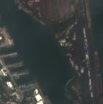
\includegraphics[width=0.9\linewidth]{figures_sentinel/sample_100_pixelside.png}
    \caption{A 100 by 100 pixel (1\,km$^2$) RGB extract from Sentinel-2.}
    \label{fig:sample_100_pixelside}
\end{figure}

\begin{figure}[ht]
    \centering
    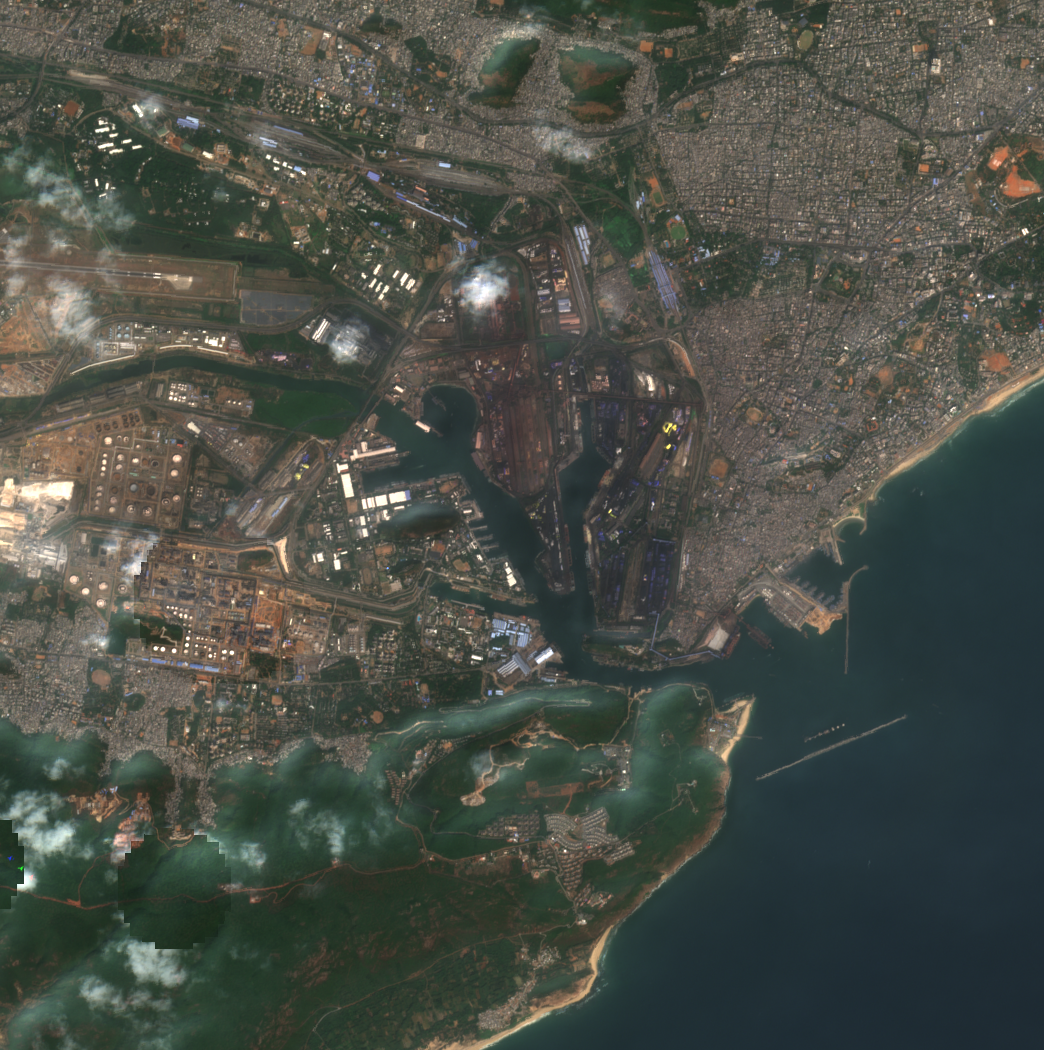
\includegraphics[width=0.9\linewidth]{figures_sentinel/sample_1000_pixelside.png}
    \caption{A 1000 by 1000 pixel (100\,km$^2$) RGB extract from Sentinel-2.}
    \label{fig:sample_1000_pixelside}
\end{figure}

\section{Training Data}

Most used seems to be forest inventory data.
Could not find much from UK Forestry.

\section{ML Estimators}

Estimators mainly in use appear to be SVM and RF. Both appear to be usable directly within the Earth Engine Python API. 

\subsection{Support Vector Machines (SVM)}

SVM works by mapping data to a high-dimensional feature space so that data points 
can be categorized, even when the data are not otherwise linearly separable.

\subsection{Random Forest (RF)}

Combines the output of multiple decision trees to reach a single result. A decision tree is a decision support hierarchical model that uses a tree-like model of decisions and their possible consequences, including chance event outcomes, resource costs, and utility.


\section{Why Classify Trees}

\begin{itemize}
    \item Broadleaved species – such as oak, beech and maple – are best because they have a larger surface area of leaves which generates more photosynthesis, whereas conifers absorb more heat. \hyperlink{https://www.glendale-services.co.uk/latest-news/plant-the-right-trees-to-combat-climate-change/}{Source.}
    \item 
\end{itemize}

\section{Tentative Literature Review}

\begin{table}[h!]
    \centering
    \caption{Sentinel-2 tree species classification literature summary.}
    \label{tab:_ex_tab}
    \begin{tabular}{lllll}     
        \toprule
        % \multicolumn{2}{c}{Bike} \\
        % \cmidrule(r){1-2}
        Literature             & Location          & Estimators   & Trees                    & S2 Bands \\
        \midrule
        \cite{germany_bavaria} & Bavaria, GER      & SVM, RF      & \makecell[l]{broad-leaved,\\ coniferous} & 8, 2, 3 \\
        \cite{china_northeast} & Northeast China   & SVM, RF, NNs & & \\
        \cite{copernicus_main} & Lower Saxony, GER & NNs          & \makecell[l]{pine, beech, spruce,\\ oak, others} & \\
        \bottomrule
    \end{tabular}
\end{table}

\section{Questions}

\begin{itemize}
    \item Surface Reflectance vs Top-of-Atmosphere Reflectance
    \item Transferability of local models
    \item Further data, e.g. NASA's \href{http://wiki.gis.com/wiki/index.php/Digital_Elevation_Model}{Digital Elevation Model}
\end{itemize}

    
    % \input{chapters/introduction.tex}
    % \input{chapters/literature.tex}% https://guides.library.bloomu.edu/litreview
    % \input{chapters/methodology.tex}
    % \chapter{Results and Validation}
\label{chapter:results}

\section{Classification Validation}

\begin{table}
\caption{Evaluation metric results, evaluation count, and training count for each tree genus.}
\label{tab:class_analysis}
\centering

\begin{tabular}{lrrrrrr}
\toprule
 & f2 score & f1 score & recall & precision & eval count & train count \\
\midrule
Pinus & 0.82 & 0.81 & 0.82 & 0.79 & 4982 & 113811 \\
Picea & 0.79 & 0.78 & 0.79 & 0.78 & 3389 & 75100 \\
Quercus & 0.75 & 0.75 & 0.74 & 0.75 & 3681 & 83306 \\
Fagus & 0.59 & 0.62 & 0.58 & 0.68 & 1528 & 34325 \\
Betula & 0.49 & 0.53 & 0.46 & 0.62 & 1840 & 40407 \\
Fraxinus & 0.25 & 0.30 & 0.22 & 0.45 & 872 & 20016 \\
Acer & 0.11 & 0.15 & 0.09 & 0.41 & 866 & 19588 \\
\bottomrule
\end{tabular}
\end{table}


\section{Change Map Correlations}

\begin{figure}[ht]
    \centering
    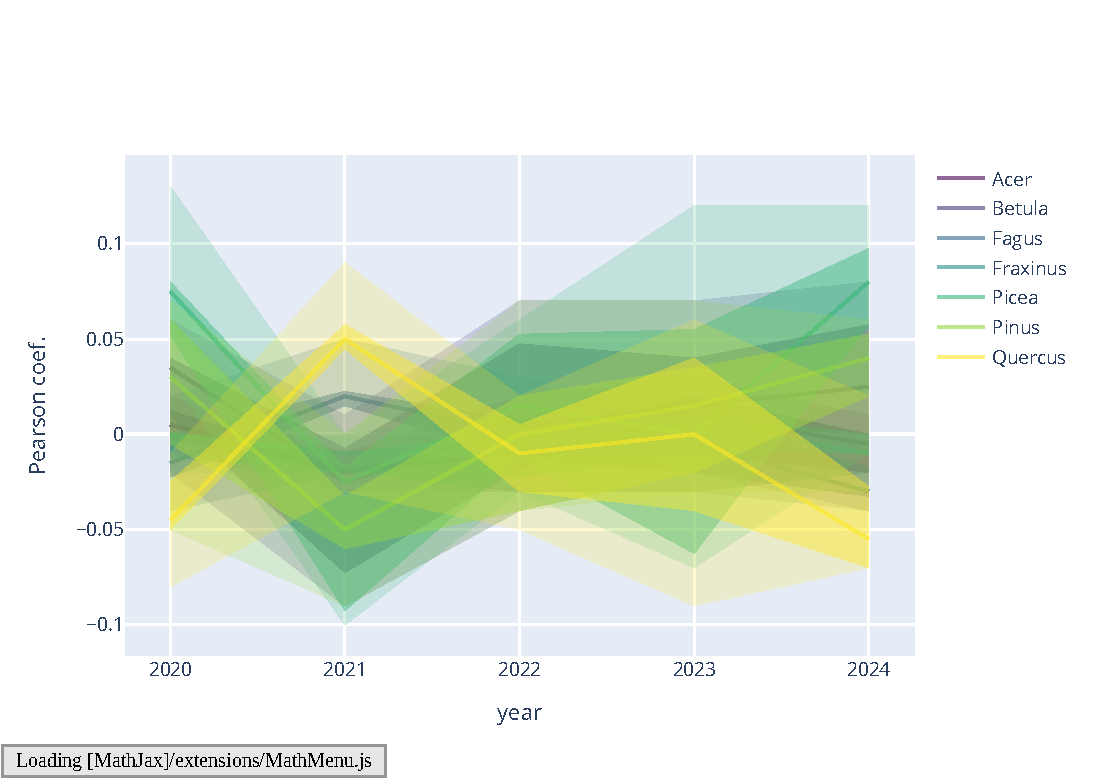
\includegraphics[width=0.98\linewidth, trim={10pt 20pt 10pt 40pt}, clip]{figures/figures_climate/genus_corr.pdf}
    \caption{Median and quantiles of Pearson correlations between changes in tree genera maps predicted by classification and differences in meteorological conditions.}
    \label{fig:genus_corr}
\end{figure}

The representative medians of the variables shown in Fig.\,\ref{fig:selected_variables_stats} were calculated for the years 2010 to 2017. The differences between these medians and those for each individual year from 2020 to 2024 were analyzed and correlated with the discrepancies between classification predictions and actual values. These results are summarized in Fig.\,\ref{fig:genus_corr}. This figure suggests that, over a short-term period of 5 years, the 7 most prominent European tree genera were not significantly affected by climate change. However, this does not account for potential long-term impacts, where even small changes could have substantial effects on ecological dynamics. Additionally, this analysis is limited to Europe, a region that may experience less pronounced climate changes compared to other parts of the world, as discussed in \cite{hoegh2018climate}. Furthermore, the study does not consider less frequent tree genera, which might be more sensitive to climate change and could exhibit different patterns of response.

\section{Relationship Modeling}

Unlike correlation, which measures the strength and direction of linear relationships between variables, relationship modeling with neural networks aims to uncover complex, non-linear interactions between variables. To further explore the relationships illustrated in Fig.\,\ref{fig:genus_corr}, a narrow, fully-connected regression neural network was developed. This network used changes in meteorological variables as predictors to analyze how these changes relate to variations in tree genera maps.

The model was trained using the Huber loss function, which combines the advantages of Mean Absolute Error (MAE) and Mean Squared Error (MSE). Huber loss is particularly effective in scenarios with noisy data and outliers, as it provides a balance between the robustness of MAE and the sensitivity to errors of MSE. 

R$^2$ was used as a primary metric because it directly measures the proportion of variance in the dependent variable that can be explained by the independent variables. This metric is particularly valuable for assessing how well the model captures the underlying relationships in the data. A higher R$^2$ value indicates a stronger relationship between the predictors and the target variable, offering insights into the effectiveness of the model in explaining variability.

MAE was chosen to evaluate the accuracy of the model's predictions. MAE provides an average of the absolute differences between the predicted and actual values, giving a clear indication of the magnitude of prediction errors. While MAE does not measure the strength of relationships directly, it helps assess how closely the model's predictions align with actual outcomes.


\begin{figure}[ht]
    \centering
    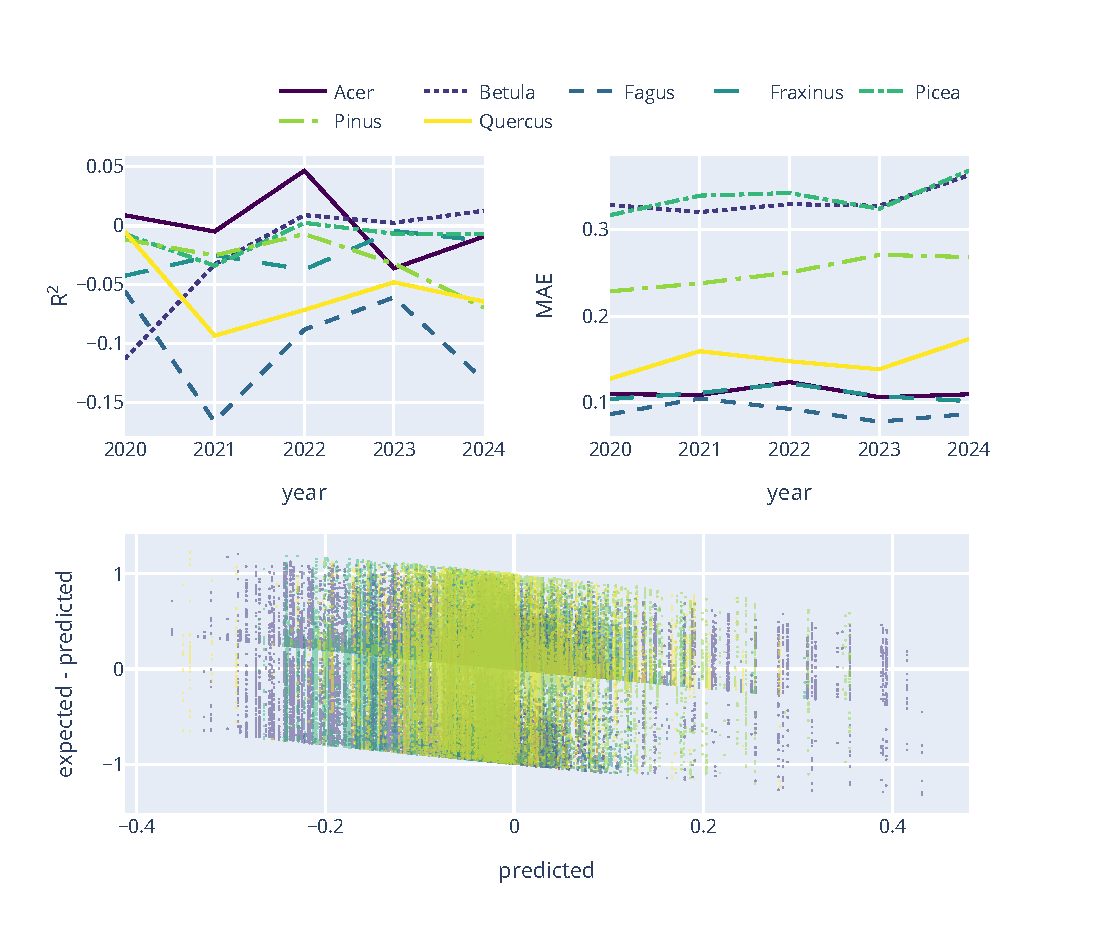
\includegraphics[width=0.98\linewidth, trim={10pt 20pt 50pt 40pt}, clip]{figures/figures_climate/regression_results.pdf}
    \caption{R$^2$ score (top-left), MAE (top-right), and residuals (bottom) for a narrow, fully-connected regression neural network, using meteorological change maps as predictors for changes in tree genus maps derived from tree classification.}
    \label{fig:regression_results}
\end{figure}

As illustrated in Fig.\,\ref{fig:regression_results}, the model exhibits a very low, and at times negative, R$^2$ value along with a high MAE. Additionally, a random sample of 50,000 residuals for the year 2024 do not display a discernible pattern, aside from clustering that reflects the original data being naturally grouped into true and false values. These results collectively indicate that the model fails to capture any significant relationship between the climate change maps and the changes in tree genus distributions. The poor performance metrics suggest that the predictors used do not meaningfully account for the variability in tree genus changes.
    % \input{chapters/discussion.tex}
    % \input{chapters/conclusions.tex}
    % \input{chapters/reflection.tex}
    

    
    % -------------------------------------------------------------------
    % Bibliography/References  -  Harvard Style was used in this report
    % -------------------------------------------------------------------
    \bibliographystyle{agsm} % Harvard Style 
    
    \bibliography{bib}  %  Patashnik, O. (1988), BibTEXing. Documentation for general BibTEX users.
    
    % -------------------------------------------------------------------
    % Appendices
    % -------------------------------------------------------------------
    
    % \begin{appendices}
    %     \input{chapters/appendix_A.tex}
    %     \input{chapters/appendix_B.tex}
    % \end{appendices}
    
\end{document}
